%  LaTeX support: latex@mdpi.com
%  Manuscript converted from the Elsevier DCN (elsarticle/ecrc) format to the
%  MDPI Symmetry template.
%=================================================================
\documentclass[symmetry,article,submit,moreauthors]{Definitions/mdpi}

%=================================================================
% MDPI internal commands - do not modify
\firstpage{1}
\makeatletter
\setcounter{page}{\@firstpage}
\makeatother
\pubvolume{1}
\issuenum{1}
\articlenumber{0}
\pubyear{2026}
\copyrightyear{2026}
\datereceived{ }
\daterevised{ }
\dateaccepted{ }
\datepublished{ }

%=================================================================
% Additional packages and definitions used by this manuscript
% (packages already loaded by mdpi.cls are not repeated here)

% mdpi.cls already defines an `algorithm' counter (for its Algorithm theorem
% environment). Undefine it so that the `algorithm' float package can be loaded.
\makeatletter
\let\c@algorithm\relax
\let\thealgorithm\relax
\makeatother
\usepackage{algorithm}
\usepackage{algpseudocode}

\usepackage{makecell}
\usepackage{listings}
\usepackage[nointegrals]{wasysym}

\newcommand{\EDHOC}{\textsf{Hybrid-EDHOC}}
\newcommand{\Hash}{\sf{H}}
\newcommand{\Extract}{\sf{Extract}}
\newcommand{\Expand}{\sf{Expand}}
\newcommand{\KDF}{\sf{KDF}}
\newcommand{\Enc}{\sf{Enc}}
\newcommand{\Dec}{\sf{Dec}}
\newcommand{\XWING}{\mathsf{X\text{-}WING}}
\newcommand{\X}{\mathsf{X}}
\newcommand{\Xtwofive}{\mathsf{X25519}}

\lstdefinestyle{proverifbox}{
  basicstyle=\ttfamily\footnotesize,
  columns=fullflexible,
  breaklines=true,
  frame=single, framerule=0.6pt, rulecolor=\color{black},
  backgroundcolor=\color{gray!1},
  numbers=none, showstringspaces=false,
  literate=
    {Verification summary:}{{{\textbf{\bfseries Verification summary:}}}}{21}
    {true.}{{{\color{green!60!black}\bfseries true.}}}6
    {false.}{{{\color{red!70!black}\bfseries false.}}}7
    {Query }{{$\bullet$~ Query }}6
}

% Status markers for the ProVerif results table
\newcommand{\statusnone}{\textcolor{red!70!black}{$\Circle$}}            % not secure
\newcommand{\statuspartial}{\textcolor{orange!80!black}{$\LEFTcircle$}}  % partial (classical only)
\newcommand{\statusfull}{\textcolor{green!60!black}{$\CIRCLE$}}          % fully secure

%=================================================================
% Full title of the paper (Capitalized)
\Title{Role-Symmetric EAP-EDHOC with Hybrid Post-Quantum Cryptography for 5G Secondary Authentication and Application-Server Access}

% Author ORCID iDs: add \orcidA{} etc. behind the author names once available
%\newcommand{\orcidauthorA}{0000-0000-0000-000X}

% Authors, for the paper (add full first names)
\Author{Adi Panca Saputra Iskandar $^{1,4}$, SeongHan Shin $^{2}$, Yongho Ko $^{1}$, I Wayan Adi Juliawan Pawana $^{1,4}$, Hoseok Kwon $^{1}$ and Ilsun You $^{1,3,}$*}

% MDPI internal command: Authors, for metadata in PDF
\AuthorNames{Adi Panca Saputra Iskandar, SeongHan Shin, Yongho Ko, I Wayan Adi Juliawan Pawana, Hoseok Kwon and Ilsun You}

% Affiliations / Addresses
\address{%
$^{1}$ \quad Department of Cybersecurity, Kookmin University, Seoul 02707, Republic of Korea; adipancaiskandar@gmail.com (A.P.S.I.); koyh0911@kookmin.ac.kr (Y.K.); adijuliawan@kookmin.ac.kr (I.W.A.J.P.)\\
$^{2}$ \quad Cyber Physical Security Research Center, National Institute of Advanced Industrial Science and Technology (AIST), Tokyo 135-0064, Japan; seonghan.shin@aist.go.jp\\
$^{3}$ \quad KMU Global Research Center for ICT Convergence Security, Kookmin University, Seoul 02707, Republic of Korea\\
$^{4}$ \quad Department of Electrical Engineering, Udayana University, Badung, Bali 80361, Indonesia}

% Contact information of the corresponding author
\corres{Correspondence: isyou@kookmin.ac.kr}

% Abstract (single paragraph, about 200 words, no blank lines)
\abstract{5G secondary authentication lets an external data network (DN) authenticate user equipment (UE) through the Extensible Authentication Protocol (EAP), but existing methods such as EAP-TLS are heavyweight and rely on elliptic-curve cryptography that a quantum adversary can break. Moving to post-quantum key encapsulation also breaks the role symmetry of authenticated key exchange, because a key encapsulation mechanism (KEM) implicitly authenticates only the decapsulating party. We propose a role-symmetric hybrid post-quantum EAP-EDHOC (Ephemeral Diffie--Hellman Over COSE) protocol that restores this symmetry: the UE and the DN authentication server each receive exactly one X-Wing (X25519 + ML-KEM-768) encapsulation to a one-time static key, each authenticate with a detached ML-DSA-44 signature, and each rotate and erase their key after every run. The mirrored rotation gives both parties forward secrecy and post-compromise security, and the independent signatures give Key-Compromise Impersonation (KCI) resistance in both directions. The exported Extended Master Session Key bootstraps application-layer keys for login-free server access. We model nine security requirements in ProVerif for seven methods, including a negative control without key erasure. An implementation on Open5GS, UERANSIM, and FreeRADIUS shows that the symmetry extends to the traffic: of the $12{,}228$-byte handshake, the UE sends $6{,}116$ bytes and the server $6{,}112$ bytes. The cost, in contrast, is asymmetric and lies in transport fragmentation and durable key storage rather than in cryptography.}

% Keywords
\keyword{symmetric mutual authentication; asymmetric cryptography; hybrid post-quantum cryptography; EDHOC; 5G secondary authentication; X-Wing KEM; ML-DSA; formal verification}

\begin{document}

%%%%%%%%%%%%%%%%%%%%%%%%%%%%%%%%%%%%%%%%%%
\section{Introduction}
\label{sec1}

A 5G operator serves many network slices and external data networks, such as enhanced mobile broadband (eMBB), ultra-reliable low-latency communication (URLLC), massive machine-type communication (mMTC), enterprise and industrial networks, and Multi-access Edge Computing (MEC). Primary authentication through 5G Authentication and Key Agreement (5G-AKA) or EAP-AKA$'$ only proves that the subscriber is legitimate for the operator and does not grant access to these services~\cite{TS33501,TS23501}. It is also not a sufficient trust anchor on its own: formal analyses of 5G-AKA have revealed protocol-level weaknesses~\cite{Edris20} and a privacy attack that survives the move from 4G to 5G~\cite{Borgaonkar19}. 5G therefore defines \emph{secondary authentication} based on the Extensible Authentication Protocol (EAP)~\cite{RFC3748,TS33501}, in which the user equipment (UE) authenticates to a data network (DN) Authentication, Authorization, and Accounting (DN-AAA) server owned by the service provider, so that connectivity is authenticated by the operator while service-level authorization stays with the service owner. Dedicated UE--DN authentication frameworks~\cite{Gong20} and analyses of the EAP-TLS profile~\cite{RFC5216,TS33501} show the growing attention paid to this step.

Figure~\ref{fig:proto-overall} places the flow in the 3GPP architecture. After primary authentication between the Access and Mobility Management Function (AMF) and the Authentication Server Function (AUSF), the UE reaches the DN-AAA server over the Session Management Function (SMF)/User Plane Function (UPF) path to run secondary authentication; the DN-AAA then bootstraps keys toward an application server (AS), using the Extended Master Session Key (EMSK), so the UE reaches the AS without a further login.

\begin{figure}[H]
\centering
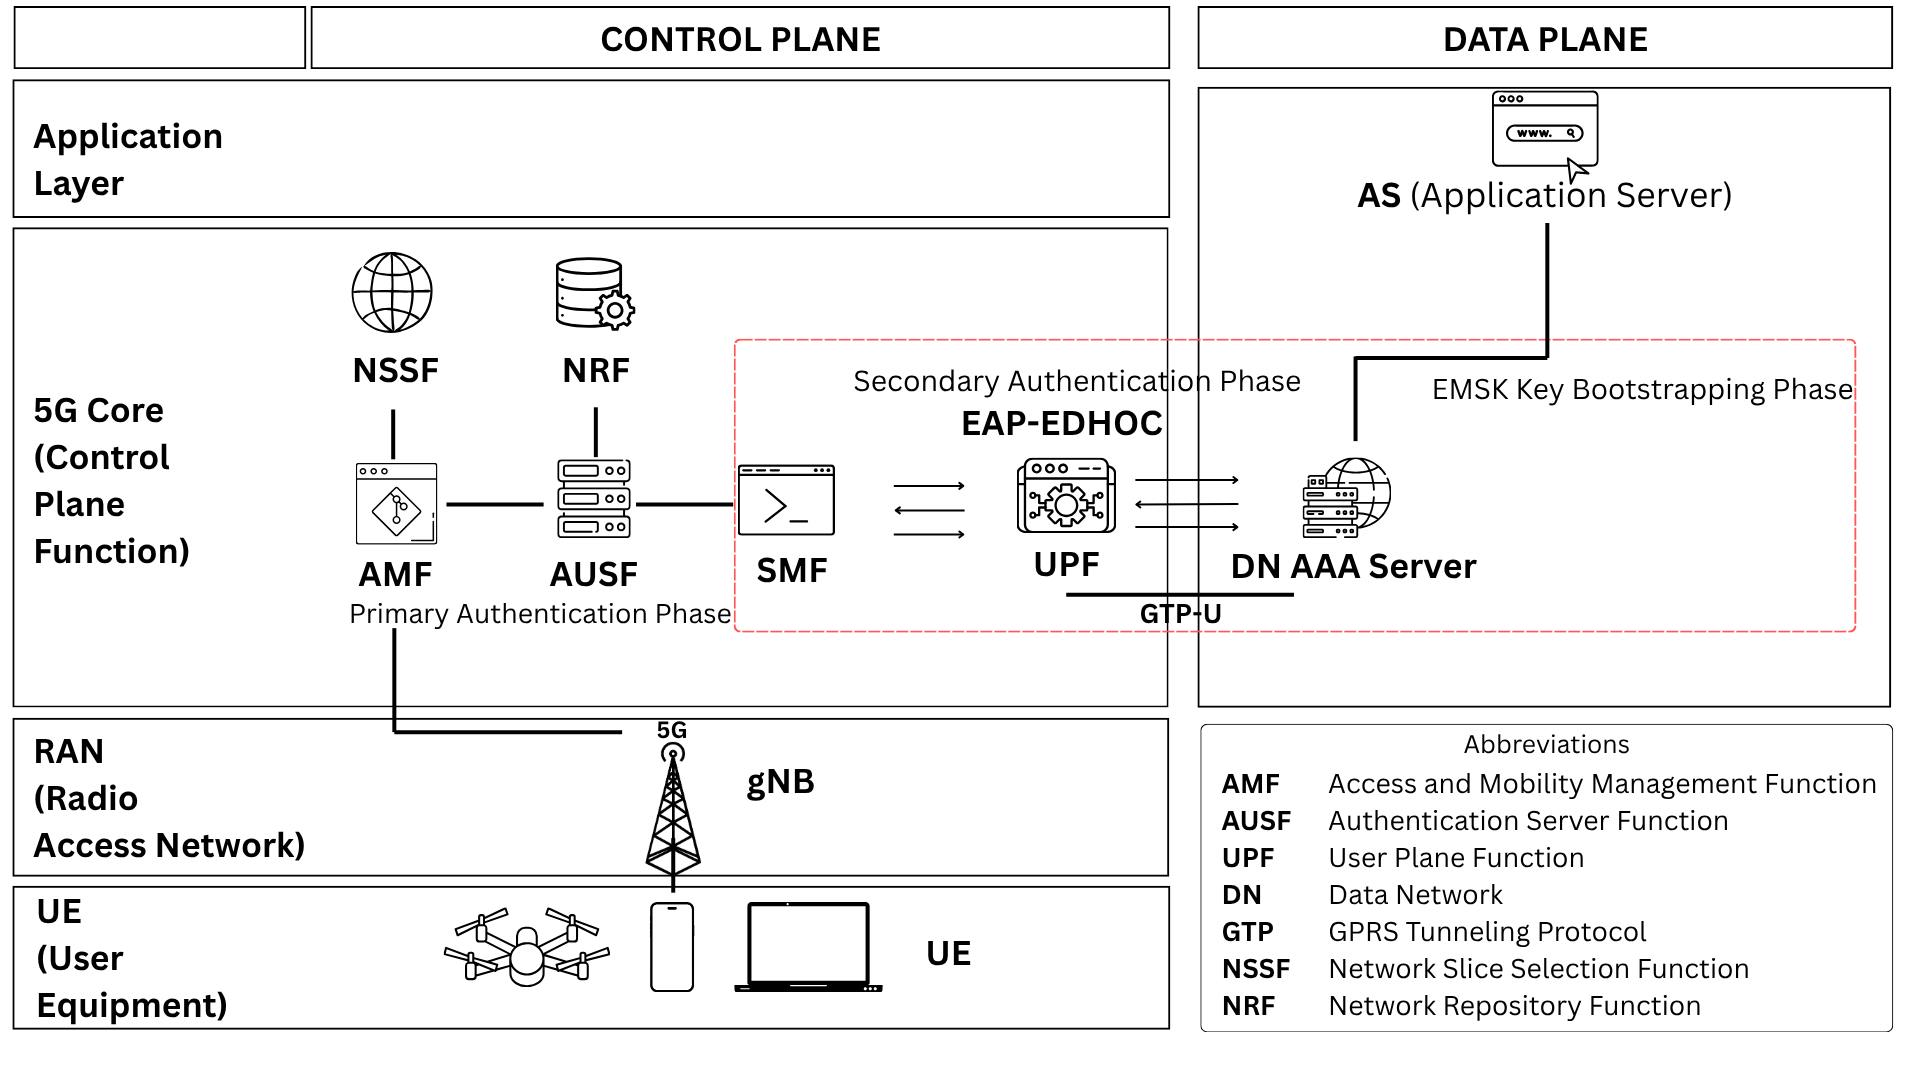
\includegraphics[width=0.85\textwidth]{img_5gFlowAuthenticationFig.png}
\caption{5G secondary authentication phase and Extended Master Session Key (EMSK) key-bootstrapping phase. AMF: Access and Mobility Management Function; AUSF: Authentication Server Function; SMF: Session Management Function; UPF: User Plane Function; DN-AAA: data network Authentication, Authorization, and Accounting server.\label{fig:proto-overall}}
\end{figure}

EAP-TLS (Transport Layer Security)~\cite{RFC5216} is costly for constrained Internet of Things (IoT) and industrial devices because of certificate exchange and the TLS handshake. EDHOC (Ephemeral Diffie--Hellman Over COSE)~\cite{RFC9528,RFC9529}, a lightweight authenticated key exchange based on the Concise Binary Object Representation (CBOR) and CBOR Object Signing and Encryption (COSE), has been carried into EAP by the EAP-EDHOC draft~\cite{EAPEDHOC} and is markedly more efficient than Datagram TLS (DTLS)~1.3~\cite{FVW24,PSM+24}. EDHOC, however, still relies on elliptic-curve Diffie--Hellman, which Shor's algorithm breaks~\cite{shor1994algorithms} and which is exposed to \emph{harvest-now, decrypt-later} attacks. Hybrid post-quantum cryptography (PQC) is the recommended transition path because it keeps interoperability with classical systems~\cite{NIST,Migration,ANSSI,PQUIP,BBF+19}; X-Wing~\cite{XWing,XWingDraft} is a compact hybrid key encapsulation mechanism (KEM) that combines X25519 with ML-KEM-768. Real hybrid-PQC deployments of EAP-EDHOC in an open-source 5G system, and the effect of PQC payloads on Remote Authentication Dial-In User Service (RADIUS) encapsulation~\cite{RFC2865,RFC3579}, remain largely unexplored~\cite{FTK+25,fraile2025reinventing,pocero,SIK+25}.

\textbf{Symmetry perspective.} Authenticated key exchange is governed by a symmetry between its two parties. Diffie--Hellman is inherently symmetric, since both sides contribute a share and derive the same secret, but a KEM is asymmetric: only the holder of the decapsulation key is implicitly authenticated. EDHOC's four methods also mix symmetric (SIG-SIG, STAT-STAT) and asymmetric, mirror-image (SIG-STAT, STAT-SIG) role assignments. Replacing Diffie--Hellman with a KEM therefore breaks the role symmetry unless the protocol restores it. Our design restores it explicitly: each party is the target of exactly one X-Wing encapsulation to a one-time static key, each party is authenticated by its own detached ML-DSA-44 signature, and each party rotates its static key after every run, which also replaces the ephemeral key pair as the source of forward secrecy. At the same time, we show that the protocol's \emph{costs} are strongly asymmetric, cheap in computation and expensive in transport, which determines where deployment effort should go.

The contributions of this work are as follows:
\begin{enumerate}
\item A role-symmetric hybrid PQC EAP-EDHOC protocol for 5G secondary authentication, built on X-Wing with a SIGMA-style ML-DSA-44 gate that resists Key-Compromise Impersonation (KCI) and a symmetric rotation of one-time static keys that provides both forward secrecy and post-compromise security without an ephemeral key pair.
\item A ProVerif~\cite{blanchet2001proverif,blanchet2016automated} analysis of nine security requirements, comparing the proposal with the four classical EDHOC methods and two EAP-TLS baselines, with a negative-control model showing that forward secrecy rests on key erasure.
\item An end-to-end implementation on Open5GS~\cite{Open5GS}, UERANSIM~\cite{UERANSIM}, and FreeRADIUS~\cite{FreeRADIUS}, with open-source code~\cite{ProVerifSrc}, including EMSK-based key bootstrapping of Object Security for Constrained RESTful Environments (OSCORE) for login-free application-server access.
\item A performance evaluation of computation, communication, EAP/RADIUS fragmentation, and packet-loss behaviour that quantifies the asymmetry between cryptographic and transport cost.
\end{enumerate}

%%%%%%%%%%%%%%%%%%%%%%%%%%%%%%%%%%%%%%%%%%
\section{Related Work}
\label{sec:relatedwork}

\textbf{Security analysis of classical EDHOC.} RFC~9528 has been analysed symbolically by Jacomme et al.~\cite{JKK+23} (all four methods), Norrman et al.~\cite{NSB21}, and Kim et al.~\cite{KDL+21}, and computationally by G\"unther and Mukendi~\cite{GM23}, Cremers et al.~\cite{CDM24}, Cottier and Pointcheval~\cite{CP22}, and Ferreira~\cite{Fer24}; P\'erez et al.~\cite{PSM+24} survey this work. A recurring finding is that the MAC-based methods (T1--T3) are vulnerable to KCI once the static Diffie--Hellman key leaks~\cite{GM23,CDM24}. These works analyse EDHOC as specified, which remains purely classical.

\textbf{Post-quantum and hybrid EDHOC.} Fraile et al.~\cite{FTK+25} propose PQ-EDHOC, a fully post-quantum variant using NIST KEMs and signatures, evaluated with microbenchmarks on constrained hardware. A companion work~\cite{fraile2025reinventing} and IETF draft~\cite{pocero} add a signature-free, KEM-based authentication method. Shin et al.~\cite{SIK+25} embed an ephemeral PQC KEM into EDHOC and omit the optional Message~4, and in follow-up work~\cite{SIK+26} they strengthen this hybrid EDHOC design toward post-quantum security against KCI. The present paper builds on that line of work and further hardens KCI resistance with a detached ML-DSA-44 gate that is independent of the KEM static keys. None of these proposals target 5G secondary authentication or integrate with EAP/RADIUS, and none combines KCI resistance with post-compromise key rotation.

\textbf{5G secondary authentication.} Gong et al.~\cite{Gong20} propose new network functions for UE--DN mutual authentication, and the EAP-TLS profile of TS~33.501 Annex~B has been formally analysed~\cite{RFC5216,TS33501}. These works do not consider PQC or the EAP-over-RADIUS fragmentation that, as we show in Section~\ref{sec:performance}, becomes the bottleneck once PQC payloads are introduced. No prior work combines hybrid PQC, a KCI-resistant gate independent of the KEM static key, formal verification, a live 5G implementation, and EMSK-based key bootstrapping.

Table~\ref{tab:methodmatrix} classifies the seven evaluated methods by the mechanism that authenticates each party. Read row by row, it exposes the role symmetry of each design: Method~0 (SIG-SIG) and Method~3 (STAT-STAT) are role-symmetric, while Methods~1 and~2 are mirror images of each other, each authenticating one party by signature and the other by a static-DH MAC. The static-DH MAC is the mechanism shown to be KCI-vulnerable~\cite{GM23,CDM24}. EAP-TLS is role-symmetric, with entity authentication provided by the \texttt{CertificateVerify} signature; its HMAC \texttt{Finished} message is a universal key-confirmation step rather than a separate authentication mechanism. Only three methods are post-quantum, and only the proposed method pairs role symmetry with a signature that is both post-quantum and detached from the key-exchange static key. Although the proposal and EAP-TLS Hybrid PQC share the same primitives, they differ in how authentication is framed, which Section~\ref{sec:performance} shows matters more for latency than the primitives themselves.

\begin{table}[H]
\caption{Cryptographic building blocks of the seven evaluated methods: the signature- or message authentication code (MAC)-based mechanism authenticating the initiator and the responder. SIG: signature; STAT: static Diffie--Hellman key; DH: Diffie--Hellman; HKDF: HMAC-based key derivation function; PQC: post-quantum cryptography.\label{tab:methodmatrix}}
\begin{adjustwidth}{-\extralength}{0cm}
\footnotesize
\begin{tabular*}{\fulllength}{@{\extracolsep{\fill}}>{\raggedright\arraybackslash}p{4.3cm}>{\raggedright\arraybackslash}p{5.4cm}>{\raggedright\arraybackslash}p{5.4cm}c@{}}
\toprule
\textbf{Method} & \textbf{Initiator authentication} & \textbf{Responder authentication} & \textbf{PQC} \\
\midrule
EAP-EDHOC Method~0 (SIG-SIG)~\cite{RFC9528,EAPEDHOC} & Signature (Ed25519) & Signature (Ed25519) & No \\
EAP-EDHOC Method~1 (SIG-STAT)~\cite{RFC9528,EAPEDHOC} & Signature (Ed25519) & Static-DH MAC (HKDF/HMAC-SHA256) & No \\
EAP-EDHOC Method~2 (STAT-SIG)~\cite{RFC9528,EAPEDHOC} & Static-DH MAC (HKDF/HMAC-SHA256) & Signature (Ed25519) & No \\
EAP-EDHOC Method~3 (STAT-STAT)~\cite{RFC9528,EAPEDHOC} & Static-DH MAC (HKDF/HMAC-SHA256) & Static-DH MAC (HKDF/HMAC-SHA256) & No \\
\textbf{EAP-EDHOC Hybrid PQC (Section~\ref{sec:eapedhocPQC}, over~\cite{EAPEDHOC})} & \textbf{Signature (ML-DSA-44, detached SIGMA gate)} & \textbf{Signature (ML-DSA-44, detached SIGMA gate)} & \textbf{Yes (hybrid)} \\
EAP-TLS Classic~\cite{RFC5216} & Signature (Ed25519, X.509 \texttt{CertificateVerify}) + HMAC \texttt{Finished} & Signature (Ed25519, X.509 \texttt{CertificateVerify}) + HMAC \texttt{Finished} & No \\
EAP-TLS Hybrid PQC~\cite{RFC5216,TLS} & Signature (ML-DSA-44, X.509 \texttt{CertificateVerify}) + HMAC \texttt{Finished} & Signature (ML-DSA-44, X.509 \texttt{CertificateVerify}) + HMAC \texttt{Finished} & Yes (hybrid) \\
\bottomrule
\end{tabular*}
\end{adjustwidth}
\end{table}

%%%%%%%%%%%%%%%%%%%%%%%%%%%%%%%%%%%%%%%%%%
\section{Preliminaries}
\label{sec:preliminaries}

\subsection{5G Secondary Authentication}
\label{sec:prelim-secondary-auth}
EAP~\cite{RFC3748} defines three roles: the \emph{peer} (the UE), the \emph{authenticator}, which relays messages without understanding the method (the SMF), and the \emph{EAP server}, which runs the method and decides (the DN-AAA)~\cite{TS33501,TS23501}. EAP frames travel over the SMF--UPF--DN-AAA path of Figure~\ref{fig:proto-overall} and are carried in RADIUS between the SMF and the DN-AAA~\cite{RFC2865,RFC3579}. Unlike primary authentication, which the AUSF terminates inside the operator's domain, secondary authentication is terminated by a DN-AAA that the operator does not control and runs only after the PDU session is established~\cite{TS33501}. A successful method exports the Master Session Key (MSK) and the Extended MSK (EMSK)~\cite{RFC3748,RFC5295}. The MSK protects the UE--DN session; the EMSK never leaves the peer and the server and serves as a root for cryptographically separated keys through RFC~5295's Usage-Specific Root Keys (USRK). We use it to bootstrap an OSCORE~\cite{RFC8613} context with an application server without any further login.

\subsection{X-Wing Hybrid KEM}
\label{sec:prelim-xwing}
X-Wing~\cite{XWing,XWingDraft} combines X25519 with ML-KEM-768 (FIPS~203)~\cite{FIPS203,CRYSTALS}, following the IETF hybrid terminology~\cite{PQUIP} and the rationale of hybrid KEMs for authenticated key exchange~\cite{BBF+19,TS103744}. The combined secret stays secure as long as \emph{at least one} component is unbroken. Algorithm~\ref{alg:xwing} summarises its three operations. The public key $pk = ek_{\mathrm{PQ}}\,\|\,pk_X$ is $1184+32$ bytes. Encapsulation runs ML-KEM-768 and an ephemeral X25519 exchange and merges both shares with a single SHA3-256 \emph{combiner} that also binds both public shares, which blocks re-encapsulation and mismatch attacks~\cite{CDM24,ADH+22}; decapsulation recomputes the same 32-byte secret.

X-Wing is IND-CCA secure under standard assumptions and, by exploiting ML-KEM's ciphertext binding, needs weaker assumptions than generic combiners~\cite{XWing}. Unlike the negotiated combiners of hybrid TLS~1.3~\cite{TLS}, IKEv2~\cite{RFC9370}, or composite ML-KEM~\cite{LAMPS,BBF+19}, it is a fixed instantiation without runtime negotiation, in line with deployed hybrids such as PQXDH~\cite{PQXDH,FG24} and post-quantum Noise~\cite{ADH+22}, and compact enough for COSE/CBOR. Note that a KEM is asymmetric by construction: the encapsulator learns nothing about the decapsulator's long-term key, and only the decapsulator is implicitly authenticated. Section~\ref{sec:symmetry} shows how the protocol compensates for this.

\begin{algorithm}[H]
\caption{X-Wing hybrid KEM: $\mathsf{KeyGen}()$, $\mathsf{Encaps}(pk)$, and $\mathsf{Decaps}(ct, sk)$}
\label{alg:xwing}
\label{alg:xwing-keygen}\label{alg:xwing-encaps}\label{alg:xwing-decaps}
{\footnotesize
\begin{algorithmic}[1]
\State \textbf{KeyGen():}
\State \hspace{1em}$(dk_{\mathrm{PQ}}, ek_{\mathrm{PQ}}) \gets \mathsf{ML\text{-}KEM\text{-}768.KeyGen}()$;\ \ $(sk_{X}, pk_{X}) \gets \Xtwofive.\mathsf{KeyGen}()$
\State \hspace{1em}\Return $pk \gets ek_{\mathrm{PQ}} \,\|\, pk_{X}$ \ ($1184 + 32 = 1216$ bytes),\ \ $sk \gets dk_{\mathrm{PQ}} \,\|\, sk_{X}$
\State \textbf{Encaps($pk = ek_{\mathrm{PQ}} \,\|\, pk_{X}$):}
\State \hspace{1em}$(ss_{\mathrm{PQ}}, ct_{\mathrm{PQ}}) \gets \mathsf{ML\text{-}KEM\text{-}768.Encaps}(ek_{\mathrm{PQ}})$;\ \ $(sk_{e}, pk_{e}) \gets \Xtwofive.\mathsf{KeyGen}()$
\State \hspace{1em}$ss_{X} \gets \Xtwofive(sk_{e}, pk_{X})$
\State \hspace{1em}$ss \gets \mathsf{SHA3\text{-}256}\big(ss_{\mathrm{PQ}} \,\|\, ss_{X} \,\|\, pk_{e} \,\|\, pk_{X} \,\|\, \texttt{label}_{\text{X-Wing}}\big)$ \Comment{combiner}
\State \hspace{1em}\Return $(ss,\ ct \gets ct_{\mathrm{PQ}} \,\|\, pk_{e})$
\State \textbf{Decaps($ct = ct_{\mathrm{PQ}} \,\|\, pk_{e}$, $sk = dk_{\mathrm{PQ}} \,\|\, sk_{X}$):}
\State \hspace{1em}$ss_{\mathrm{PQ}} \gets \mathsf{ML\text{-}KEM\text{-}768.Decaps}(ct_{\mathrm{PQ}}, dk_{\mathrm{PQ}})$;\ \ $ss_{X} \gets \Xtwofive(sk_{X}, pk_{e})$
\State \hspace{1em}\Return $ss \gets \mathsf{SHA3\text{-}256}\big(ss_{\mathrm{PQ}} \,\|\, ss_{X} \,\|\, pk_{e} \,\|\, pk_{X} \,\|\, \texttt{label}_{\text{X-Wing}}\big)$
\end{algorithmic}
}
\end{algorithm}

%%%%%%%%%%%%%%%%%%%%%%%%%%%%%%%%%%%%%%%%%%
\section{Proposed EAP-EDHOC Hybrid PQC Protocol}
\label{sec:eapedhocPQC}

\subsection{Assumptions and Design Rationale}
In a provisioning phase (Algorithm~\ref{alg:longterm-keygen}), the UE (Initiator) and the DN-AAA (Responder) each generate a long-term X-Wing key pair and a long-term ML-DSA-44 signing key, and each holds the peer's long-term X-Wing public key. The peer's verification key ($VK_R$, $VK_I$) is conveyed in \texttt{Plaintext2}/\texttt{Plaintext3} and bound to the transcript by the corresponding signature. EAP-EDHOC messages are carried over EAP~\cite{RFC3748} and RADIUS~\cite{RFC2865,RFC3579} between the pass-through authenticator (SMF/UPF) and the DN-AAA, following TS~33.501~\cite{TS33501}. The Dolev--Yao adversary~\cite{DolevYao1983} controls the network.

The X-Wing static keys are \emph{one-time} keys. Each party generates its next key pair during a run, announces the public key in $\mathit{EAD}_3$ or $\mathit{EAD}_4$, and erases the old secret key once the run completes, so every static key pair serves exactly one session. The DN-AAA therefore keeps one record per UE, holding $(sk_{\mathsf{B}}, pk_{\mathsf{B}})$ for that UE together with $(pk_{\mathsf{A}}, VK_I)$. The DN-AAA selects this record from the EAP identity of the session, which reaches it in the RADIUS Access-Request before \texttt{Message1}, so no extra field is added to the EDHOC messages.

The protocol follows the SIGMA (SIGn-and-MAc) design~\cite{Kra03}: X-Wing provides confidentiality and key agreement, while detached ML-DSA-44 signatures~\cite{FIPS204} are the sole source of entity authentication. Because the signing keys are independent of the X-Wing static keys, leaking a KEM static key does not enable impersonation; this closes the KCI gap of a MAC-only Method~4 variant~\cite{GM23,CDM24}. We choose ML-DSA-44 (NIST category~2) rather than ML-DSA-65 to limit fragmentation: its $1312$-byte key and $2420$-byte signature are markedly smaller, and its margin still exceeds that of the Ed25519 signatures of T0--T3. Being nominally below the category-3 strength of ML-KEM-768, this is a deliberate size/security trade-off.

\begin{algorithm}[H]
\caption{Long-term key generation (provisioning)}
\label{alg:longterm-keygen}
{\footnotesize
\begin{algorithmic}[1]
\State \textbf{At UE:}\ \ $(sk_{\mathsf{A}}, pk_{\mathsf{A}}) \gets \XWING.\mathsf{KeyGen}()$;\ \ $(sk_{\mathsf{SIG,I}}, VK_I) \gets \mathsf{ML\text{-}DSA\text{-}44.KeyGen}()$
\State \textbf{At DN-AAA:}\ \ $(sk_{\mathsf{B}}, pk_{\mathsf{B}}) \gets \XWING.\mathsf{KeyGen}()$;\ \ $(sk_{\mathsf{SIG,R}}, VK_R) \gets \mathsf{ML\text{-}DSA\text{-}44.KeyGen}()$
\State \Return $(pk_{\mathsf{A}}, sk_{\mathsf{A}}, sk_{\mathsf{SIG,I}}, VK_I),\ (pk_{\mathsf{B}}, sk_{\mathsf{B}}, sk_{\mathsf{SIG,R}}, VK_R)$
\end{algorithmic}
}
\end{algorithm}

\subsection{Handshake}
Figure~\ref{fig:proto-edhoc} shows the exchange inside the 3GPP secondary-authentication flow, with the SMF as EAP authenticator and the DN-AAA as EAP server reached over RADIUS.

\begin{figure}[H]
\begin{adjustwidth}{-\extralength}{0cm}
\centering
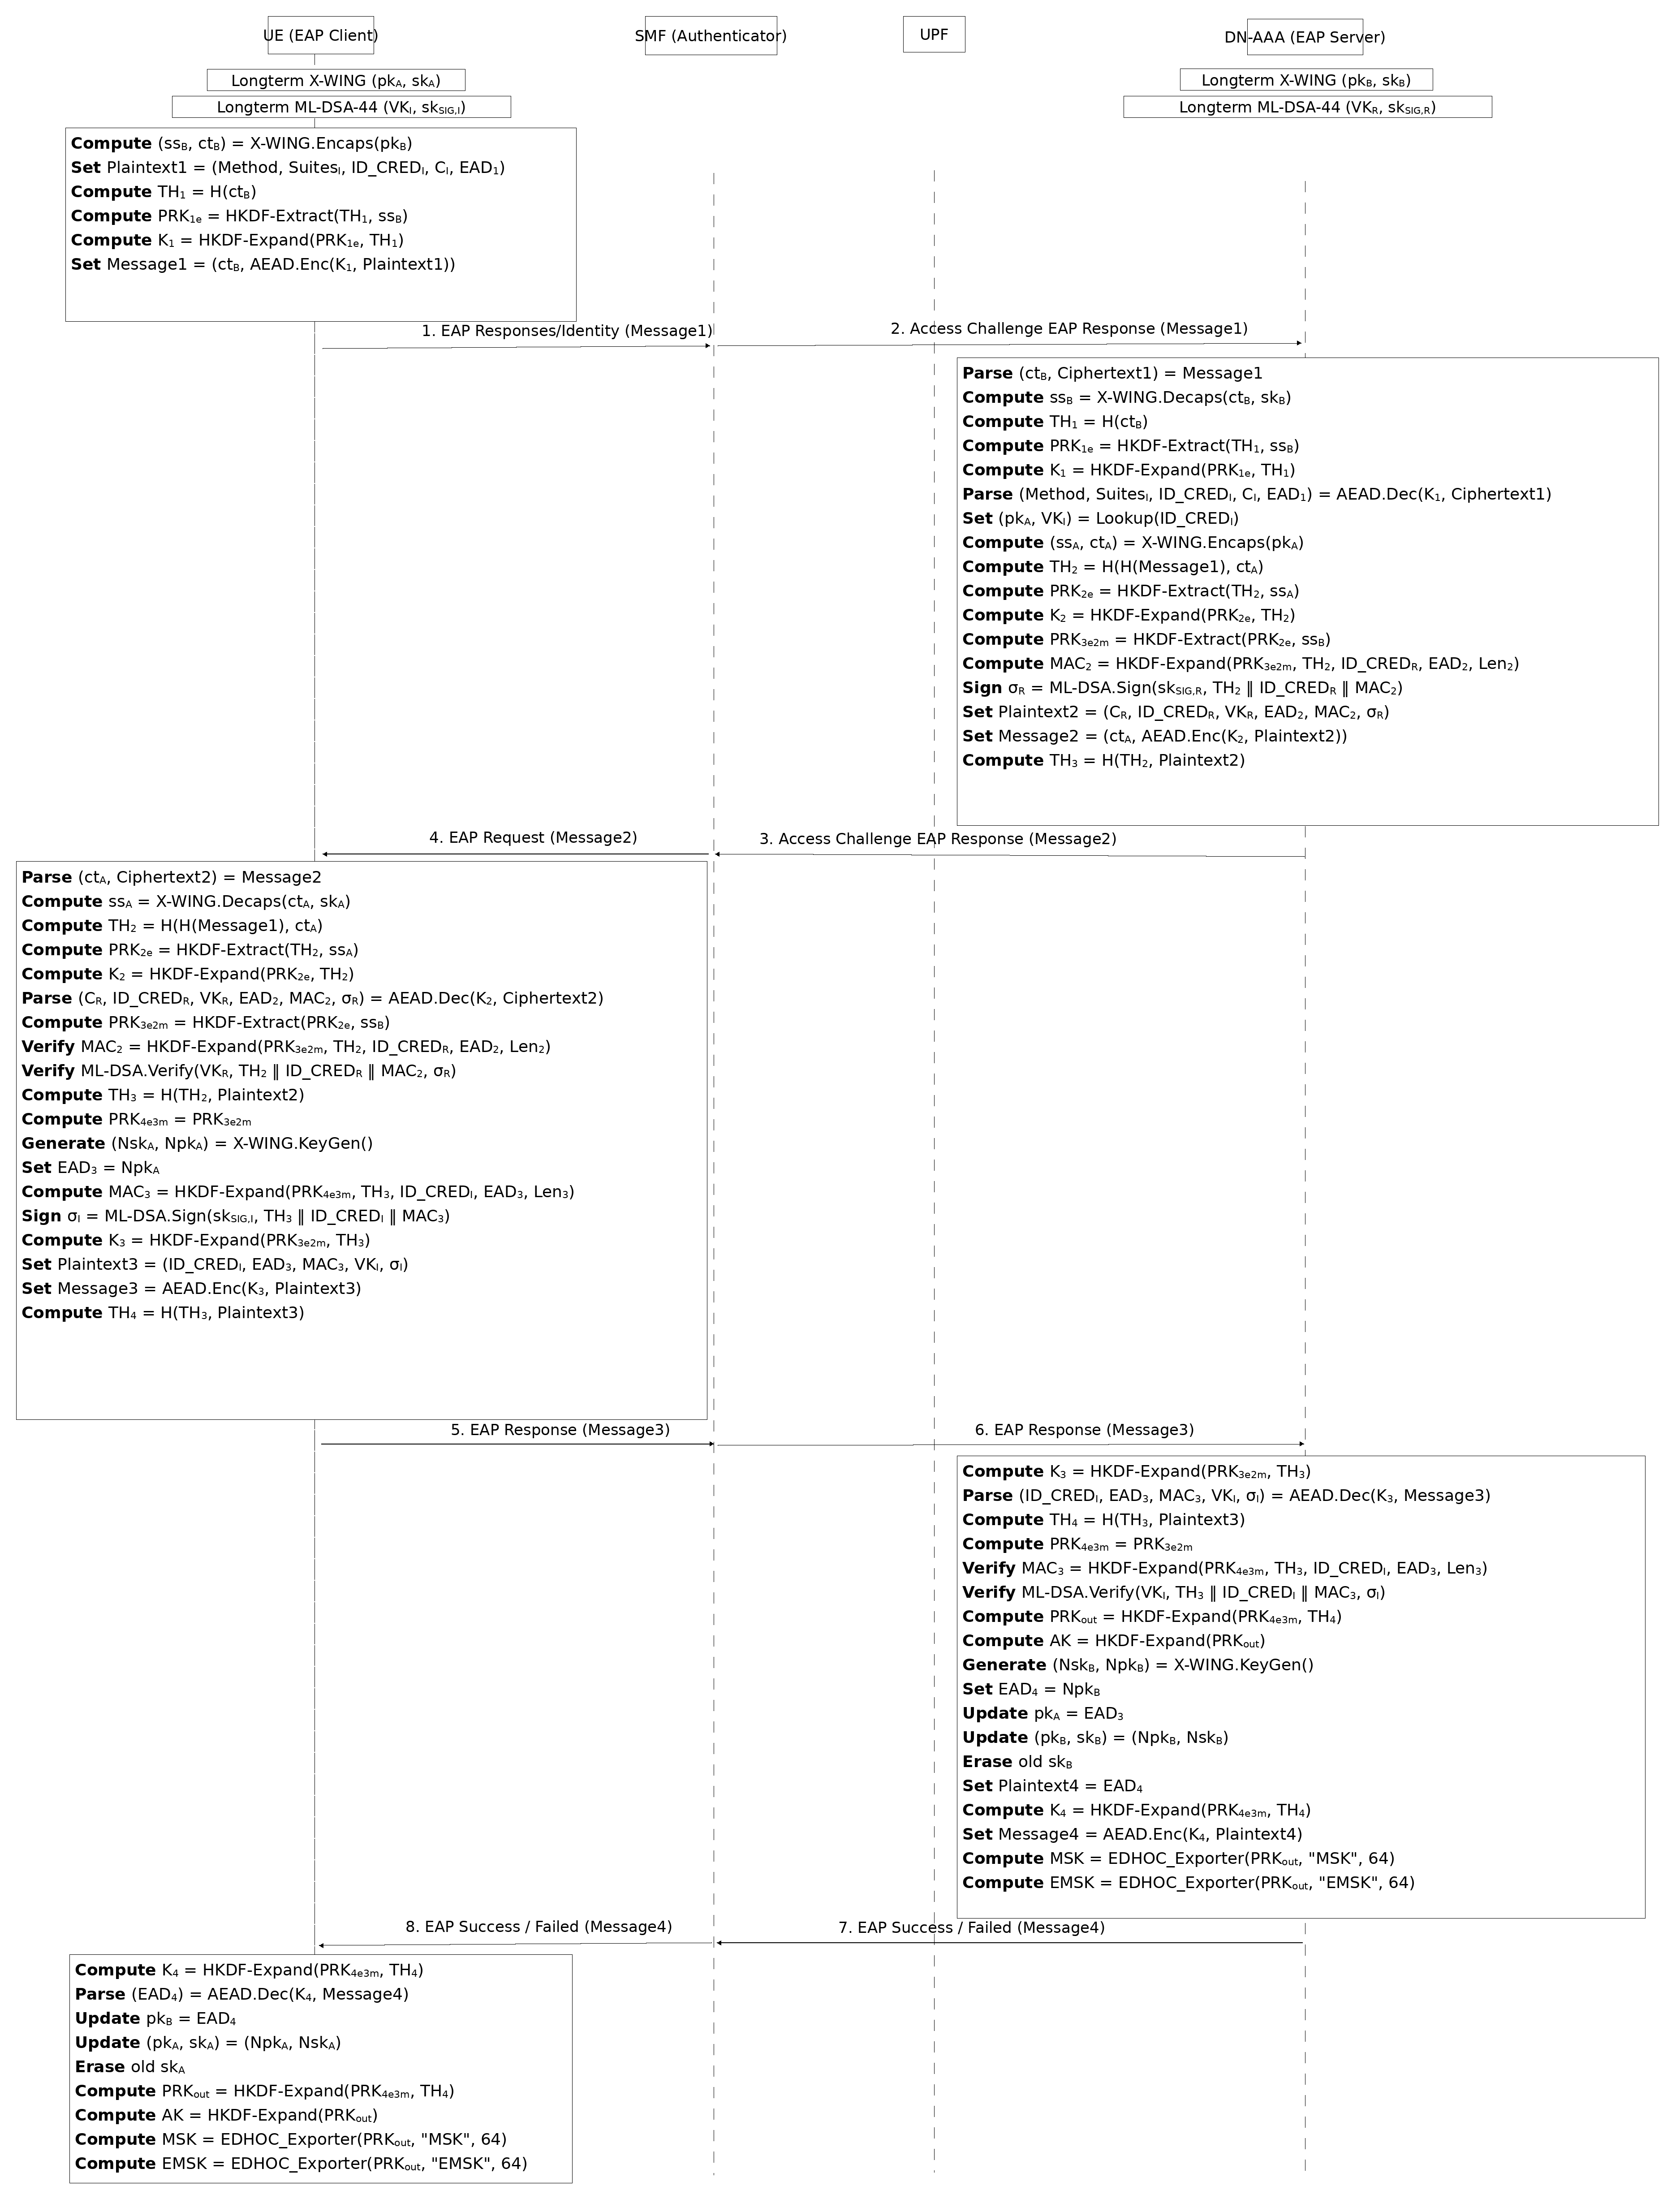
\includegraphics[width=\linewidth,height=0.8\textheight,keepaspectratio]{img_SecondaryAuth2_v2.png}
\end{adjustwidth}
\caption{EAP-EDHOC hybrid PQC protocol for 5G secondary authentication.\label{fig:proto-edhoc}}
\end{figure}

\textbf{Message~1} (Algorithm~\ref{alg:message1}). The UE encapsulates a fresh secret to the DN-AAA's current one-time key $pk_B$ and encrypts \texttt{Plaintext1} under a transcript-derived key $K_1$. No ephemeral key pair is generated: forward secrecy comes from the erasure of the one-time static keys (Section~\ref{sec:symmetry}). \texttt{Plaintext1} carries $\mathit{ID\_CRED}_I$ so that the DN-AAA can retrieve $pk_A$ before building \texttt{Message2}. Because $K_1$ depends only on $ss_B$, $\mathit{ID\_CRED}_I$ is exposed if the \emph{current} $sk_B$ is compromised before the run; once the run completes and $sk_B$ is erased, a later compromise no longer reveals it, which Section~\ref{sec:formalverif} checks formally.

\begin{algorithm}[H]
\caption{Construction of \texttt{Message1} (Initiator)}
\label{alg:message1}
{\footnotesize
\begin{algorithmic}[1]
\Require $pk_{\mathsf{B}} \text{ (current one-time public key of the DN-AAA)}$
\Ensure $\mathsf{Message1}$
\State $(ss_{\mathsf{B}}, ct_{\mathsf{B}}) \gets \XWING.\mathsf{Encaps}(pk_{\mathsf{B}})$
\State $\mathsf{Plaintext1} \gets (\mathsf{Method}, \mathsf{Suites}_I, \mathit{ID\_CRED}_I, C_I, \mathsf{EAD}_1)$
\State $TH_1 \gets H(ct_{\mathsf{B}})$
\State $PRK_{1e} \gets \mathsf{HKDF\text{-}Extract}(TH_1, ss_{\mathsf{B}})$
\State $K_1 \gets \mathsf{HKDF\text{-}Expand}(PRK_{1e}, TH_1)$
\State $\mathsf{Message1} \gets \big(ct_{\mathsf{B}},\ \mathsf{AEAD.Enc}(K_1, \mathsf{Plaintext1})\big)$
\State \Return $\mathsf{Message1}$
\end{algorithmic}
}
\end{algorithm}

\textbf{Message~2} (Algorithm~\ref{alg:message2}). Using the UE record selected from the EAP identity, the DN-AAA decapsulates, retrieves $(pk_A, VK_I)$ from $\mathit{ID\_CRED}_I$, and encapsulates to the UE's one-time key $pk_A$. The ciphertext $ct_A$ travels in the clear part of \texttt{Message2}, and $ss_A$ keys the encryption of \texttt{Plaintext2}, so the Responder's identity is readable only by the holder of $sk_A$. The DN-AAA signs $TH_2\,\|\,\mathit{ID\_CRED}_R\,\|\,\mathit{MAC}_2$ with a key independent of $sk_B$, giving KCI-resistant Responder authentication.

\begin{algorithm}[H]
\caption{EDHOC \texttt{Message2} (DN-AAA $\to$ UE) with ML-DSA-44 authentication}
\label{alg:message2}
{\footnotesize
\begin{algorithmic}[1]
\Require $\mathsf{Message1},\ \text{per-UE records},\ sk_{\mathsf{SIG,R}},\ VK_R$
\Ensure $\mathsf{Message2}$
\State $(ct_{\mathsf{B}}, \mathsf{Ciphertext1}) \gets \mathsf{Message1}$
\State $ss_{\mathsf{B}} \gets \XWING.\mathsf{Decaps}(ct_{\mathsf{B}}, sk_{\mathsf{B}})$
\State $TH_1 \gets H(ct_{\mathsf{B}})$
\State $PRK_{1e} \gets \mathsf{HKDF\text{-}Extract}(TH_1, ss_{\mathsf{B}})$
\State $K_1 \gets \mathsf{HKDF\text{-}Expand}(PRK_{1e}, TH_1)$
\State $(\mathsf{Method}, \mathsf{Suites}_I, \mathit{ID\_CRED}_I, C_I, \mathsf{EAD}_1) \gets \mathsf{AEAD.Dec}(K_1, \mathsf{Ciphertext1})$
\State $(pk_{\mathsf{A}}, VK_I) \gets \mathsf{Lookup}(\mathit{ID\_CRED}_I)$
\State $(ss_{\mathsf{A}}, ct_{\mathsf{A}}) \gets \XWING.\mathsf{Encaps}(pk_{\mathsf{A}})$
\State $TH_2 \gets H\big(H(\mathsf{Message1}),\ ct_{\mathsf{A}})$
\State $PRK_{2e} \gets \mathsf{HKDF\text{-}Extract}(TH_2, ss_{\mathsf{A}})$
\State $K_2 \gets \mathsf{HKDF\text{-}Expand}(PRK_{2e}, TH_2)$
\State $PRK_{3e2m} \gets \mathsf{HKDF\text{-}Extract}(PRK_{2e}, ss_{\mathsf{B}})$
\State $\mathit{MAC}_2 \gets \mathsf{HKDF\text{-}Expand}\big(PRK_{3e2m}, TH_2, \mathit{ID\_CRED}_R, \mathit{EAD}_2, \mathit{Len}_2\big)$
\State $\sigma_R \gets \mathsf{ML\text{-}DSA.Sign}\big(sk_{\mathsf{SIG,R}},\ TH_2 \,\|\, \mathit{ID\_CRED}_R \,\|\, \mathit{MAC}_2\big)$ \Comment{\textbf{independent of $sk_{\mathsf{B}}$}}
\State $\mathsf{Plaintext2} \gets (C_R, \mathit{ID\_CRED}_R, VK_R, \mathit{EAD}_2, \mathit{MAC}_2, \sigma_R)$
\State $\mathsf{Message2} \gets \big(ct_{\mathsf{A}},\ \mathsf{AEAD.Enc}(K_2, \mathsf{Plaintext2})\big)$
\State $TH_3 \gets H(TH_2, \mathsf{Plaintext2})$
\State \Return $\mathsf{Message2}$
\end{algorithmic}
}
\end{algorithm}

\textbf{Message~3} (Algorithm~\ref{alg:message3}). The UE verifies $\mathit{MAC}_2$ and $\sigma_R$; this signature check is an authentication \emph{gate} that must pass before the handshake continues. The UE then authenticates itself in the mirror-image manner and announces a fresh X-Wing public key $\mathit{Npk}_{\mathsf{A}}$ in $\mathit{EAD}_3$.

\begin{algorithm}[H]
\caption{EDHOC \texttt{Message3} (UE $\to$ DN-AAA), KCI-resistant via the ML-DSA-44 gate}
\label{alg:message3}
{\footnotesize
\begin{algorithmic}[1]
\Require $\mathsf{Message2},\ sk_{\mathsf{A}},\ ss_{\mathsf{B}},\ sk_{\mathsf{SIG,I}},\ VK_I$
\Ensure $\mathsf{Message3}$
\State $(ct_{\mathsf{A}}, \mathsf{Ciphertext2}) \gets \mathsf{Message2}$
\State $ss_{\mathsf{A}} \gets \XWING.\mathsf{Decaps}(ct_{\mathsf{A}}, sk_{\mathsf{A}})$
\State $TH_2 \gets H\big(H(\mathsf{Message1}),\ ct_{\mathsf{A}})$
\State $PRK_{2e} \gets \mathsf{HKDF\text{-}Extract}(TH_2, ss_{\mathsf{A}})$
\State $K_2 \gets \mathsf{HKDF\text{-}Expand}(PRK_{2e}, TH_2)$
\State $(C_R, \mathit{ID\_CRED}_R, VK_R, \mathit{EAD}_2, \mathit{MAC}_2, \sigma_R) \gets \mathsf{AEAD.Dec}(K_2, \mathsf{Ciphertext2})$
\State $PRK_{3e2m} \gets \mathsf{HKDF\text{-}Extract}(PRK_{2e}, ss_{\mathsf{B}})$
\State \textbf{Verify} $\mathit{MAC}_2 \overset{?}{=} \mathsf{HKDF\text{-}Expand}(PRK_{3e2m}, TH_2, \mathit{ID\_CRED}_R, \mathit{EAD}_2, \mathit{Len}_2)$ \Comment{key confirmation}
\State \textbf{Verify} $\mathsf{ML\text{-}DSA.Verify}\big(VK_R,\ TH_2 \,\|\, \mathit{ID\_CRED}_R \,\|\, \mathit{MAC}_2,\ \sigma_R\big) \overset{?}{=} \mathtt{valid}$ \Comment{\textbf{auth gate}}
\State \textbf{if either check fails:} \textbf{abort}
\State $TH_3 \gets H(TH_2, \mathsf{Plaintext2})$
\State $PRK_{4e3m} \gets PRK_{3e2m}$ \Comment{$ss_{\mathsf{A}}$ already entered at $PRK_{2e}$}
\State $(\mathit{Nsk}_{\mathsf{A}}, \mathit{Npk}_{\mathsf{A}}) \gets \XWING.\mathsf{KeyGen}()$;\ \ $\mathit{EAD}_3 \gets \mathit{Npk}_{\mathsf{A}}$
\State $\mathit{MAC}_3 \gets \mathsf{HKDF\text{-}Expand}(PRK_{4e3m}, TH_3, \mathit{ID\_CRED}_I, \mathit{EAD}_3, \mathit{Len}_3)$
\State $\sigma_I \gets \mathsf{ML\text{-}DSA.Sign}\big(sk_{\mathsf{SIG,I}},\ TH_3 \,\|\, \mathit{ID\_CRED}_I \,\|\, \mathit{MAC}_3\big)$ \Comment{\textbf{independent of $sk_{\mathsf{A}}$}}
\State $K_3 \gets \mathsf{HKDF\text{-}Expand}(PRK_{3e2m}, TH_3)$
\State $\mathsf{Plaintext3} \gets (\mathit{EAD}_3, \mathit{MAC}_3, VK_I, \sigma_I)$
\State $\mathsf{Message3} \gets \mathsf{AEAD.Enc}(K_3, \mathsf{Plaintext3})$
\State $TH_4 \gets H(TH_3, \mathsf{Plaintext3})$
\State \Return $\mathsf{Message3}$
\end{algorithmic}
}
\end{algorithm}

\textbf{Message~4 and key export} (Algorithms~\ref{alg:message4} and~\ref{alg:message4-export}). The DN-AAA verifies the Initiator's gate, finalises the key schedule, rotates its own key pair, erases the old secret key, and returns a fresh $\mathit{Npk}_{\mathsf{B}}$ in $\mathit{EAD}_4$. The UE processes \texttt{Message4}, and both endpoints export identical MSK and EMSK with the EDHOC exporter. The MSK is returned to the 5G core; the EMSK is retained for key bootstrapping.

\begin{algorithm}[H]
\caption{EDHOC \texttt{Message4} (DN-AAA $\to$ UE), KCI-resistant via the ML-DSA-44 gate}
\label{alg:message4}
{\footnotesize
\begin{algorithmic}[1]
\Require $\mathsf{Message3},\ PRK_{3e2m},\ TH_3$
\Ensure $\mathsf{Message4}$
\State $K_3 \gets \mathsf{HKDF\text{-}Expand}(PRK_{3e2m}, TH_3)$
\State $(\mathit{EAD}_3, \mathit{MAC}_3, VK_I, \sigma_I) \gets \mathsf{AEAD.Dec}(K_3, \mathsf{Message3})$
\State $TH_4 \gets H(TH_3, \mathsf{Plaintext3})$
\State $PRK_{4e3m} \gets PRK_{3e2m}$
\State \textbf{Verify} $\mathit{MAC}_3 \overset{?}{=} \mathsf{HKDF\text{-}Expand}(PRK_{4e3m}, TH_3, \mathit{ID\_CRED}_I, \mathit{EAD}_3, \mathit{Len}_3)$ \Comment{key confirmation}
\State \textbf{Verify} $\mathsf{ML\text{-}DSA.Verify}\big(VK_I,\ TH_3 \,\|\, \mathit{ID\_CRED}_I \,\|\, \mathit{MAC}_3,\ \sigma_I\big) \overset{?}{=} \mathtt{valid}$ \Comment{\textbf{auth gate}}
\State \textbf{if either check fails:} \textbf{abort}
\State $PRK_{\mathsf{out}} \gets \mathsf{HKDF\text{-}Expand}(PRK_{4e3m}, TH_4)$;\ \ $AK \gets \mathsf{HKDF\text{-}Expand}(PRK_{\mathsf{out}})$
\State $(\mathit{Nsk}_{\mathsf{B}}, \mathit{Npk}_{\mathsf{B}}) \gets \XWING.\mathsf{KeyGen}()$;\ \ $\mathit{EAD}_4 \gets \mathit{Npk}_{\mathsf{B}}$
\State $pk_{\mathsf{A}} \gets \mathit{EAD}_3$ \Comment{update next key of UE}
\State $(pk_{\mathsf{B}}, sk_{\mathsf{B}}) \gets (\mathit{Npk}_{\mathsf{B}}, \mathit{Nsk}_{\mathsf{B}})$;\ \ \textbf{erase} the old $sk_{\mathsf{B}}$ \Comment{forward secrecy}
\State $\mathsf{Plaintext4} \gets \mathit{EAD}_4$;\ \ $K_4 \gets \mathsf{HKDF\text{-}Expand}(PRK_{4e3m}, TH_4)$
\State $\mathsf{Message4} \gets \mathsf{AEAD.Enc}(K_4, \mathsf{Plaintext4})$
\State $\mathrm{MSK} \gets \mathtt{EDHOC\_Exporter}(PRK_{\mathsf{out}}, \text{``MSK''}, 64)$;\ \ $\mathrm{EMSK} \gets \mathtt{EDHOC\_Exporter}(PRK_{\mathsf{out}}, \text{``EMSK''}, 64)$
\State \Return $\mathsf{Message4}$
\end{algorithmic}
}
\end{algorithm}

\begin{algorithm}[H]
\caption{\texttt{Message4} processing and session-key export (UE)}
\label{alg:message4-export}
{\footnotesize
\begin{algorithmic}[1]
\Require $\mathsf{Message4},\ PRK_{4e3m},\ TH_4$
\Ensure $\mathrm{MSK},\ \mathrm{EMSK}$
\State $K_4 \gets \mathsf{HKDF\text{-}Expand}(PRK_{4e3m}, TH_4)$;\ \ $(\mathit{EAD}_4) \gets \mathsf{AEAD.Dec}(K_4, \mathsf{Message4})$
\State $pk_{\mathsf{B}} \gets \mathit{EAD}_4$ \Comment{update next key of DN-AAA}
\State $(pk_{\mathsf{A}}, sk_{\mathsf{A}}) \gets (\mathit{Npk}_{\mathsf{A}}, \mathit{Nsk}_{\mathsf{A}})$;\ \ \textbf{erase} the old $sk_{\mathsf{A}}$ \Comment{forward secrecy}
\State $PRK_{\mathsf{out}} \gets \mathsf{HKDF\text{-}Expand}(PRK_{4e3m}, TH_4)$;\ \ $AK \gets \mathsf{HKDF\text{-}Expand}(PRK_{\mathsf{out}})$
\State $\mathrm{MSK} \gets \mathtt{EDHOC\_Exporter}(PRK_{\mathsf{out}}, \text{``MSK''}, 64)$;\ \ $\mathrm{EMSK} \gets \mathtt{EDHOC\_Exporter}(PRK_{\mathsf{out}}, \text{``EMSK''}, 64)$
\State \Return $(\mathrm{MSK}, \mathrm{EMSK})$
\end{algorithmic}
}
\end{algorithm}

\begin{figure}[H]
\begin{adjustwidth}{-\extralength}{0cm}
\centering
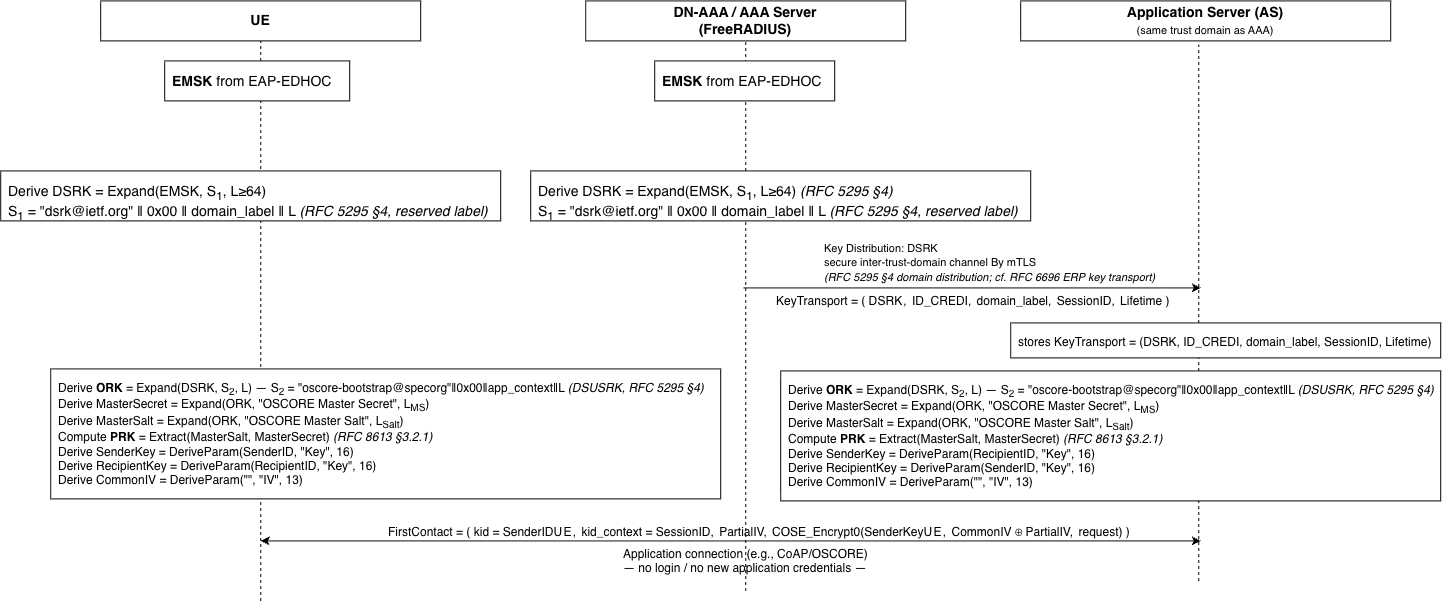
\includegraphics[width=\linewidth]{img_phase-key-bootstrapping.png}
\end{adjustwidth}
\caption{Application-server access through key bootstrapping from the EMSK.\label{fig:proto-bootstrap}}
\end{figure}

\subsection{EMSK-Based Key Bootstrapping}
Once secondary authentication succeeds, the UE and the DN-AAA share an identical EMSK. Figure~\ref{fig:proto-bootstrap} shows how it bootstraps keys that let the UE access the AS directly, and Figure~\ref{fig:proto-keysched} gives the key schedule, which combines RFC~5295's root-key hierarchy~\cite{RFC5295} with the OSCORE security context of RFC~8613~\cite{RFC8613}. Every arrow is a single $\mathsf{Expand}$ or $\mathsf{Extract}$ call with a unique label, so compromise of one derived key does not disclose keys at another level (cryptographic separation, RFC~5295 Section~3). This phase uses only symmetric-key primitives, so its cost is negligible next to the asymmetric handshake that precedes it (Section~\ref{sec:perf-bootstrap}).

\begin{figure}[H]
\centering
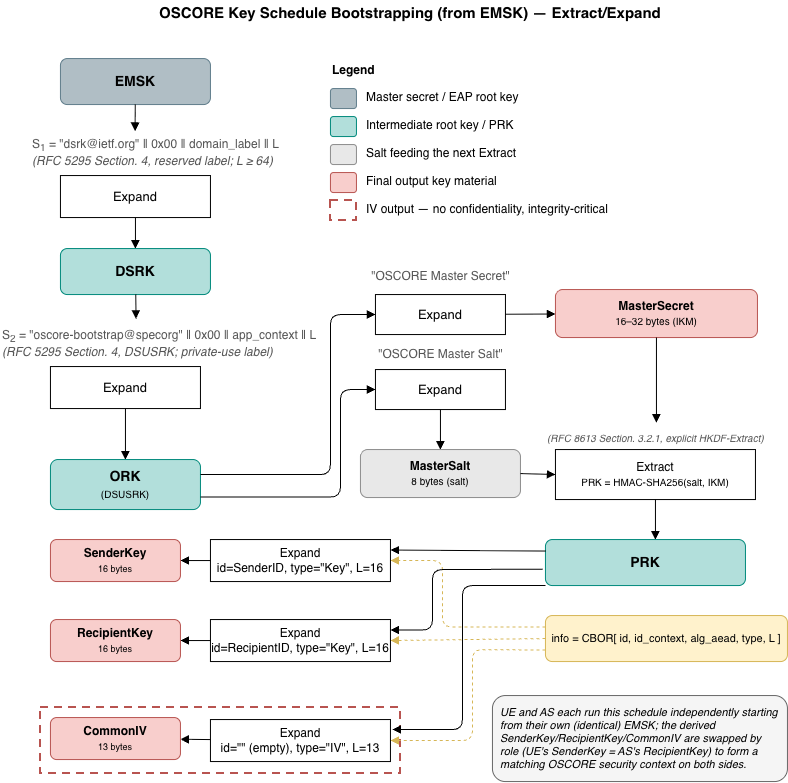
\includegraphics[width=0.72\textwidth]{img_KeyscheduleEMSKBootstrapingKey.png}
\caption{Key schedule for bootstrapping keys from the EMSK.\label{fig:proto-keysched}}
\end{figure}

\subsection{Symmetry Analysis of the Design}
\label{sec:symmetry}
We call a protocol \emph{role-symmetric} if exchanging the Initiator and the Responder maps each party's cryptographic obligations onto those of the other. The proposed protocol satisfies this property in four respects, summarised in Table~\ref{tab:symmetry}.

\emph{(i) Symmetric implicit authentication through two encapsulations.} A single KEM authenticates only the decapsulator. The protocol therefore performs exactly two encapsulations, one in each direction: $ct_B$ to the DN-AAA in \texttt{Message1} and $ct_A$ to the UE in \texttt{Message2}. Both secrets feed the key schedule ($ss_A$ into $PRK_{2e}$, $ss_B$ into $PRK_{3e2m}$), and each message is encrypted under the secret it delivers to its receiver, $K_1$ from $ss_B$ and $K_2$ from $ss_A$. This reproduces, with an asymmetric primitive, the two-sided contribution that static Diffie--Hellman gives naturally.

\emph{(ii) Symmetric explicit authentication.} Each party signs its own transcript hash with a detached ML-DSA-44 key ($\sigma_R$ over $TH_2$, $\sigma_I$ over $TH_3$), and each verification is a mandatory gate. In contrast to the mirror-image methods T1/T2, neither party relies on a static-DH MAC, so KCI resistance holds for both directions rather than for one.

\emph{(iii) Symmetric key rotation.} The UE announces $\mathit{Npk}_{\mathsf{A}}$ in $\mathit{EAD}_3$ and the DN-AAA announces $\mathit{Npk}_{\mathsf{B}}$ in $\mathit{EAD}_4$; both replace their static key at the end of the run and erase the old secret key. Because every static key pair therefore serves a single session, this two-sided rotation yields forward secrecy (R\ref{req:fs}) as well as post-compromise security for both parties (R\ref{req:pcs}), without an ephemeral key pair.

\emph{(iv) Symmetric key confirmation and output.} $\mathit{MAC}_2$ and $\mathit{MAC}_3$ give mutual key confirmation, and both ends derive identical MSK/EMSK values.

The design keeps two intentional asymmetries. First, \texttt{Message1} must carry $\mathit{ID\_CRED}_I$ so that the Responder can select $pk_A$; the Initiator's identity is therefore protected only under the Responder's \emph{current} one-time key (R\ref{req:idconceal}). Second, the four-message flow is not size-symmetric, as \texttt{Message2} and \texttt{Message3} carry the signatures and verification keys. The total bytes sent in each direction are nevertheless balanced: $6{,}116$~B from the UE (\texttt{Message1}+\texttt{Message3}) and $6{,}112$~B from the DN-AAA (\texttt{Message2}+\texttt{Message4}).

\begin{table}[H]
\caption{Role symmetry of the proposed protocol: corresponding obligations of the Initiator (UE) and the Responder (DN-AAA).\label{tab:symmetry}}
\footnotesize
\begin{tabular*}{\textwidth}{@{\extracolsep{\fill}}>{\raggedright\arraybackslash}p{3.3cm}>{\raggedright\arraybackslash}p{4.3cm}>{\raggedright\arraybackslash}p{4.3cm}@{}}
\toprule
\textbf{Obligation} & \textbf{Initiator (UE)} & \textbf{Responder (DN-AAA)} \\
\midrule
Static encapsulation received & $ct_A$ to $pk_A$ (in \texttt{Message2}) & $ct_B$ to $pk_B$ (in \texttt{Message1}) \\
Secret fed to key schedule & $ss_A \to PRK_{2e}$ & $ss_B \to PRK_{3e2m}$ \\
Key-confirmation MAC sent & $\mathit{MAC}_3$ & $\mathit{MAC}_2$ \\
Detached signature (gate) & $\sigma_I$ over $TH_3$, verified by DN-AAA & $\sigma_R$ over $TH_2$, verified by UE \\
Static-key rotation and erasure & $\mathit{Npk}_{\mathsf{A}}$ in $\mathit{EAD}_3$, old $sk_A$ erased & $\mathit{Npk}_{\mathsf{B}}$ in $\mathit{EAD}_4$, old $sk_B$ erased \\
Session-key output & MSK, EMSK & MSK, EMSK \\
\midrule
Intentional asymmetry & $\mathit{ID\_CRED}_I$ sent under the current $pk_B$-derived key & --- \\
\bottomrule
\end{tabular*}
\end{table}

%%%%%%%%%%%%%%%%%%%%%%%%%%%%%%%%%%%%%%%%%%
\section{Formal Security Verification Using ProVerif}
\label{sec:formalverif}

We analyse the protocol with ProVerif~\cite{blanchet2001proverif,blanchet2016automated} in the Dolev--Yao model~\cite{DolevYao1983,dolev1983security}, following prior EDHOC analyses~\cite{JKK+23,NSB21,KDL+21,Fer24,cremers2017symbolic} and ISO/IEC~29128~\cite{ISO29128}. The verification targets nine requirements:
\begin{enumerate}[label=R\arabic*,ref=\arabic*,leftmargin=2.6em]
\item \label{req:mutualauth} \textbf{Mutual authentication}: each party is injectively authenticated to the other (agreement on the transcript).
\item \label{req:idconceal} \textbf{Identity concealment}: the persistent identities $\mathit{ID\_CRED}_I$ and $\mathit{ID\_CRED}_R$ are not learned by the adversary.
\item \label{req:confidentiality} \textbf{Confidentiality}: application data and session keys remain secret.
\item \label{req:keyexchange} \textbf{Secure key exchange}: MSK/EMSK are secret and agreed.
\item \label{req:fs} \textbf{Forward secrecy}: past session keys remain secret when the long-term state held after the session (signing keys and current static keys) leaks.
\item \label{req:pcs} \textbf{Post-compromise security}: after a static key is compromised, security is restored once the rotated $\mathit{Npk}_{\mathsf{A}}/\mathit{Npk}_{\mathsf{B}}$ is in use.
\item \label{req:aead} \textbf{AEAD protection} (Authenticated Encryption with Associated Data): plaintexts are integrity- and confidentiality-protected.
\item \label{req:qr} \textbf{Quantum resilience}: security holds against an adversary that can solve discrete logarithms, i.e., when X25519 and Ed25519 are broken (modelled by a quantum oracle).
\item \label{req:kci} \textbf{KCI resistance}: compromise of a party's static KEM key does not allow impersonation of the peer.
\end{enumerate}

Table~\ref{tab:verification-query} maps each requirement to its ProVerif queries. We model seven variants: EDHOC T0 (SIG-SIG), T1 (SIG-STAT), T2 (STAT-SIG), T3 (STAT-STAT), the proposed protocol, and the two EAP-TLS baselines of Section~\ref{sec:performance}, which are modelled as certificate-authenticated TLS~1.3 handshakes over the same query set. Each variant is analysed in three settings. In the \emph{classical} setting, an active Dolev--Yao attacker controls the network and, in phase~1, learns all long-term keys of both parties. The \emph{quantum} setting adds an oracle, available in every phase, that returns the discrete logarithm of any X25519 element and the Ed25519 signing key of any Ed25519 public key; this models Shor's algorithm against both an active attacker and recorded traffic, while no such oracle exists for ML-KEM-768 or ML-DSA-44. In the \emph{KCI} setting, the long-term keys of one party are known to the attacker from the start, and we check that its peer is still authenticated to it. X-Wing is modelled with its two halves kept separate: either secret half opens only its own component of a ciphertext, the shared secret needs both, and the quantum oracle recovers only the X25519 half, so the quantum setting checks the hybrid property instead of assuming it. Post-compromise security is checked in a dedicated model of the proposed protocol: after a run, the old static X-Wing keys of both parties are revealed, and a second run under the keys rotated through $\mathit{EAD}_3$/$\mathit{EAD}_4$ is analysed. A property is fully secure (\statusfull) if it holds in both the classical and the quantum setting, and partial (\statuspartial) if it holds only in the classical setting. For the proposed protocol, each run uses a fresh one-time static key pair per party, and the state leaked in phase~1 is the state a device actually holds after the run: the rotated X-Wing keys and both ML-DSA-44 signing keys. A negative-control model (\texttt{edhoc\_m4v2\_fs\_noerase.pv}) additionally leaks the old, unerased keys; there the forward-secrecy and identity queries must fail, which shows that these properties rest on key erasure and that the models are not trivially secure. All 23 models target ProVerif~2.05; the models, run scripts, and outputs are publicly available~\cite{ProVerifSrc}.

\begin{table}[H]
\caption{Security requirements and verification queries.\label{tab:verification-query}}
\begin{adjustwidth}{-\extralength}{0cm}
\footnotesize
\begin{tabular*}{\fulllength}{@{\extracolsep{\fill}}l l@{}}
\toprule
\textbf{Security Requirement} & \textbf{Verification Query} \\
\midrule
\multirow{4}{*}{Mutual authentication (R\ref{req:mutualauth})}
 & Q1: \texttt{event(UE\_send\_M1(M1))} \\
 & Q2: \texttt{inj-event(UE\_recv\_M2(...))} $\Rightarrow$ \texttt{inj-event(DN\_send\_M2(...))} \\
 & Q3: \texttt{inj-event(DN\_recv\_M3(...))} $\Rightarrow$ \texttt{inj-event(UE\_send\_M3(...))} \\
 & Q4: \texttt{inj-event(UE\_recv\_M4(...))} $\Rightarrow$ \texttt{inj-event(DN\_send\_M4(...))} \\
\midrule
Identity concealment (R\ref{req:idconceal}) & Q5: \texttt{attacker(ID\_CREDI)};\ \ Q5b: \texttt{attacker(ID\_CREDR)} \\
\midrule
\multirow{2}{*}{Confidentiality (R\ref{req:confidentiality})} & Q6: \texttt{attacker(app\_data\_UE)} \\
 & Q7: \texttt{attacker(app\_data\_DN)} \\
\midrule
\multirow{2}{*}{Secure key exchange (R\ref{req:keyexchange})} & Q8: \texttt{attacker(MSK\_test)} \\
 & Q9: \texttt{attacker(EMSK\_test)} \\
\midrule
Forward secrecy (R\ref{req:fs}) & Q8 \&\& Q9 after \texttt{phase 1} leaks the post-run state; no-erasure control must fail \\
\midrule
Post-compromise security (R\ref{req:pcs}) & Q10: \texttt{attacker(MSK\_test2)} \&\& Q11: \texttt{attacker(EMSK\_test2)} after the old static keys are revealed \\
\midrule
AEAD protection (R\ref{req:aead}) & Q2 \&\& Q3 \&\& Q4 (implicit via the \texttt{AEAD\_dec} rewrite) \\
\midrule
Quantum resilience (R\ref{req:qr}) & Q8 \&\& Q9 in the quantum setting (X25519 discrete-log and Ed25519 key-recovery oracle) \\
\midrule
KCI resistance (R\ref{req:kci}) & Q2 \&\& Q4 with the UE's long-term keys leaked; Q3 with the DN's long-term keys leaked \\
\bottomrule
\end{tabular*}
\end{adjustwidth}
\end{table}

Figure~\ref{fig:proverif-transcript} shows the condensed ProVerif output. The reachability query (\texttt{is false}) is a sanity check that honest runs complete. The three injective correspondences (\texttt{is true}) confirm mutual authentication with transcript agreement for both directions of the handshake (R\ref{req:mutualauth}), which formally reflects the role symmetry of Section~\ref{sec:symmetry}. The \texttt{attacker\_p1} queries confirm that, even after the static keys leak, the adversary learns neither the application data (R\ref{req:confidentiality}) nor MSK/EMSK (R\ref{req:keyexchange}, R\ref{req:fs}), and the key-rotation model confirms that a later session under the rotated keys regains secrecy (Q10, Q11; R\ref{req:pcs}). Because the protocol has no ephemeral key pair, rotation with erasure is also what provides forward secrecy: the state leaked after a run holds only the next one-time keys, which never protected that run. As the leaked state no longer contains the erased one-time keys, neither $\mathit{ID\_CRED}_I$ (Q5) nor $\mathit{ID\_CRED}_R$ (Q5b) is revealed; in the negative control, which keeps the old keys, Q5, Q5b, and Q6--Q9 fail, so forward secrecy and identity concealment rest on erasure. The negative control queries only secrecy: its extra keys leak in phase 1, after every authentication event, so its Q2--Q4 coincide with those of the classical model. Because authentication rests on signatures independent of the KEM static keys, leaking $sk_A/sk_B$ breaks neither authentication nor KCI resistance (R\ref{req:kci}); replacing the static-DH MAC of a Method~4 variant~\cite{GM23,CDM24} with a SIGMA-style signature is precisely what removes this exposure.

\begin{figure}[H]
\begin{lstlisting}[style=proverifbox]
Verification summary:
 Query not event(UE_send_M1(W0,m))                      is false.
 Query inj-event(UE_recv_M2(W0,x,t))
       ==> inj-event(DN_send_M2(W0,x,t))                is true.
 Query inj-event(DN_recv_M3(W0,x,t))
       ==> inj-event(UE_send_M3(W0,x,t))                is true.
 Query inj-event(UE_recv_M4(W0,x,t))
       ==> inj-event(DN_send_M4(W0,x,t))                is true.
 Query not attacker_p1(ID_CREDI[])                      is true.
 Query not attacker_p1(ID_CREDR[])                      is true.
 Query not attacker_p1(app_data_UE[])                   is true.
 Query not attacker_p1(app_data_DN[])                   is true.
 Query not attacker_p1(MSK_test[])                      is true.
 Query not attacker_p1(EMSK_test[])                     is true.
 Query not attacker(MSK_test2[])                        is true.
 Query not attacker(EMSK_test2[])                       is true.
\end{lstlisting}
\caption{ProVerif verification summary for the proposed protocol: Q1--Q9 from \texttt{edhoc\_m4v2\_classical.pv} and Q10--Q11 from the key-rotation model (\texttt{edhoc\_m4v2\_pcs.pv}).\label{fig:proverif-transcript}}
\end{figure}

Table~\ref{tab:proverif-results} compares all seven variants. The classical methods T0--T3 and EAP-TLS Classic reach R\ref{req:mutualauth}--R\ref{req:fs}, R\ref{req:aead}, and R\ref{req:kci} only against a classical adversary and fail R\ref{req:pcs} and R\ref{req:qr}: in their quantum-setting models, every authentication and secrecy query turns false, whereas all queries of the two hybrid variants keep their classical verdicts. EAP-TLS Hybrid PQC, which uses the same X25519MLKEM768 group and ML-DSA-44 certificates, retains its guarantees against a quantum adversary, consistent with the composition argument for hybrid combiners~\cite{BBF+19,XWing} and the EUF-CMA security of ML-DSA-44~\cite{FIPS204}, and with published TLS~1.3 analyses~\cite{cremers2017symbolic}. Like every other variant, however, it fails post-compromise security, because TLS~1.3 defines no static-key rotation. The T0--T3 and EAP-TLS models follow their specifications exactly, so their \statusnone\ on R\ref{req:pcs} reflects the absence of a rotation step in the standards rather than an inherent impossibility. The proposed protocol is the only variant that is fully secure on all nine requirements, with forward secrecy and identity concealment conditional on key erasure.

\begin{table}[H]
\caption{ProVerif verification results across EDHOC authentication methods and the two EAP-TLS baselines.\label{tab:proverif-results}}
\begin{adjustwidth}{-\extralength}{0cm}
\footnotesize
\begin{tabular*}{\fulllength}{@{\extracolsep{\fill}}>{\raggedright\arraybackslash}p{3.6cm}ccccccc@{}}
\toprule
\textbf{Security Requirement} & \makecell{\textbf{EAP-EDHOC}\\\textbf{Method 0}\\\footnotesize\cite{RFC9528,EAPEDHOC}} & \makecell{\textbf{EAP-EDHOC}\\\textbf{Method 1}\\\footnotesize\cite{RFC9528,EAPEDHOC}} & \makecell{\textbf{EAP-EDHOC}\\\textbf{Method 2}\\\footnotesize\cite{RFC9528,EAPEDHOC}} & \makecell{\textbf{EAP-EDHOC}\\\textbf{Method 3}\\\footnotesize\cite{RFC9528,EAPEDHOC}} & \makecell{\textbf{EAP-}\\\textbf{EDHOC}\\\textbf{Hybrid}\\\footnotesize(Sec.~\ref{sec:eapedhocPQC})} & \makecell{\textbf{EAP-TLS}\\\textbf{Classic}\\\footnotesize\cite{RFC5216}} & \makecell{\textbf{EAP-TLS}\\\textbf{Hybrid PQC}\\\footnotesize\cite{RFC5216,TLS}} \\
\midrule
R\ref{req:mutualauth} Mutual authentication    & \statuspartial & \statuspartial & \statuspartial & \statuspartial & \statusfull & \statuspartial & \statusfull \\
R\ref{req:idconceal} Identity concealment      & \statuspartial & \statuspartial & \statuspartial & \statuspartial & \statusfull$^{\dagger}$ & \statuspartial & \statusfull \\
R\ref{req:confidentiality} Confidentiality     & \statuspartial & \statuspartial & \statuspartial & \statuspartial & \statusfull & \statuspartial & \statusfull \\
R\ref{req:keyexchange} Secure key exchange     & \statuspartial & \statuspartial & \statuspartial & \statuspartial & \statusfull & \statuspartial & \statusfull \\
R\ref{req:fs} Forward secrecy                  & \statuspartial & \statuspartial & \statuspartial & \statuspartial & \statusfull & \statuspartial & \statusfull \\
R\ref{req:pcs} Post-compromise security        & \statusnone & \statusnone & \statusnone & \statusnone & \statusfull & \statusnone & \statusnone \\
R\ref{req:aead} AEAD protection                & \statuspartial & \statuspartial & \statuspartial & \statuspartial & \statusfull & \statuspartial & \statusfull \\
R\ref{req:qr} Quantum resilience               & \statusnone & \statusnone & \statusnone & \statusnone & \statusfull & \statusnone & \statusfull \\
R\ref{req:kci} KCI resistance                  & \statuspartial & \statuspartial & \statuspartial & \statuspartial & \statusfull & \statuspartial & \statusfull \\
\bottomrule
\end{tabular*}
\noindent{\footnotesize{\statusnone\ not secure; \statuspartial\ partial (secure only against a classical adversary); \statusfull\ fully secure (classical \emph{and} quantum adversary). Every entry is a ProVerif result, except the \statusnone\ marks on R\ref{req:pcs} for the six baselines, whose specifications define no static-key rotation. $^{\dagger}$$\mathit{ID\_CRED}_I$ is sent in \texttt{Message1} under a key derived from the DN-AAA's current one-time key. It stays secret after that key is erased, but is exposed if the current $sk_B$ is compromised before the run.}}
\end{adjustwidth}
\end{table}

%%%%%%%%%%%%%%%%%%%%%%%%%%%%%%%%%%%%%%%%%%
\section{Performance Evaluation}
\label{sec:performance}

\subsection{Testbed and Cryptographic Cost}
Experiments ran on a Windows 11 Pro host (Intel Core i9-14900K, 64\,GB DDR5) in a VirtualBox VM with Ubuntu 24.04 LTS (16\,GB RAM, 12 vCPUs). The testbed uses Open5GS~\cite{Open5GS}, UERANSIM~\cite{UERANSIM}, and FreeRADIUS~\cite{FreeRADIUS}, all co-located in the VM and communicating over loopback, so the measured network overhead reflects protocol-stack, scheduling, and RADIUS processing rather than RAN/WAN propagation and should be read as a lower bound. We modified Open5GS~2.7.2, UERANSIM~3.2.7, and FreeRADIUS~3.2.6. The EDHOC methods (0--4) use libsodium~\cite{libsodium} for X25519, Ed25519, SHA-256, and HKDF, mbedTLS~\cite{mbedtls} for AES-128-GCM (both from the Ubuntu 24.04 LTS repositories), and the PQClean~\cite{pqclean} clean reference implementations of ML-KEM-768 and ML-DSA-44. The EAP-TLS baselines use OpenSSL: EAP-TLS Classic runs on the system OpenSSL~3.0.13, while EAP-TLS Hybrid PQC runs on a separately built OpenSSL~3.2.6 with liboqs~0.16~\cite{liboqs} and oqs-provider~0.12~\cite{openssl_oqs}, because ML-DSA-44 certificates in TLS~1.3 require OpenSSL~3.2 or later; each Hybrid PQC handshake is checked at run time to have negotiated the X25519MLKEM768 group and an ML-DSA-44 certificate. The source code, configuration, and benchmark scripts are publicly available~\cite{ProVerifSrc}. EAP-EDHOC runs over real EAP-over-RADIUS (RFC~2865/3579)~\cite{RFC2865,RFC3579} to a FreeRADIUS \texttt{rlm\_eap\_edhoc} responder along the path UE $\to$ AMF $\to$ SMF $\to$ UPF $\to$ FreeRADIUS. All five EDHOC methods are implemented: methods 0--3 use three messages and method~4 (the proposal) four messages with EAP fragmentation. EAP-TLS Classic and EAP-TLS Hybrid PQC are benchmarked end to end on the same testbed.

During the preparation of this manuscript, the authors used Claude (Anthropic; model claude-opus-5-5) to convert the manuscript to the journal template and to condense and restructure the text; the tool was not used to generate data, results, or analyses. The authors reviewed and edited the output and take full responsibility for the content of this publication.

Table~\ref{tab:primitive} lists primitive costs over $3000$ iterations. The most expensive operation, ML-DSA-44 signing, averages $0.223$~ms, and all ML-KEM-768 operations stay below $0.05$~ms. Per handshake, the proposed method costs $0.985$~ms, split exactly evenly between the initiator and the responder ($0.492$~ms each): apart from generating its next key pair, each party performs exactly one X-Wing encapsulation and one decapsulation, one signature and one verification, so the two parties run mirror-image operation sets. The classical methods 0--3 cost $0.152$--$0.182$~ms, and EAP-TLS Classic and Hybrid PQC $0.182$~ms and $0.775$~ms. PQC thus multiplies computation by about $5$--$6.5\times$, yet the absolute cost stays below $1$~ms. Figures~\ref{fig:handshake_computation_grouped} and~\ref{fig:communication_breakdown_methods} break down computation and communication for all seven methods.

\begin{table}[H]
\caption{Mean latency of cryptographic primitives (3000 iterations).\label{tab:primitive}}
\footnotesize
\begin{tabular*}{\textwidth}{@{\extracolsep{\fill}}lrrr@{}}
\toprule
\textbf{Operation} & \textbf{Mean (ms)} & \textbf{StdDev (ms)} & \textbf{95\% CI ($\pm$ms)} \\
\midrule
Keygen\_X25519      & 0.025535 & 0.029916 & 0.001071 \\
ScalarMult\_X25519  & 0.025164 & 0.019026 & 0.000681 \\
Keygen\_Ed25519     & 0.010730 & 0.017312 & 0.000619 \\
Signature\_Ed25519  & 0.011070 & 0.010091 & 0.000361 \\
Verify\_Ed25519     & 0.029439 & 0.020345 & 0.000728 \\
SHA256              & 0.000300 & 0.001233 & 0.000044 \\
HKDF\_SHA256        & 0.001456 & 0.005022 & 0.000180 \\
AES128GCM           & 0.000226 & 0.000021 & 0.000001 \\
Keygen\_MLKEM768    & 0.032440 & 0.024176 & 0.000865 \\
Encaps\_MLKEM768    & 0.033775 & 0.019317 & 0.000691 \\
Decaps\_MLKEM768    & 0.041870 & 0.021982 & 0.000787 \\
Keygen\_MLDSA44     & 0.056854 & 0.041449 & 0.001483 \\
Signature\_MLDSA44  & 0.223241 & 0.212971 & 0.007621 \\
Verify\_MLDSA44     & 0.059596 & 0.028310 & 0.001013 \\
\bottomrule
\end{tabular*}
\end{table}

\begin{figure}[H]
\begin{adjustwidth}{-\extralength}{0cm}
\centering

\includegraphics[width=\linewidth]{img_handshake_computation_grouped.png}
\end{adjustwidth}
\caption{Per-method handshake computation cost (\textbf{left}) and end-to-end handshake time (\textbf{right}).\label{fig:handshake_computation_grouped}}
\end{figure}

\begin{figure}[H]
\begin{adjustwidth}{-\extralength}{0cm}
\centering
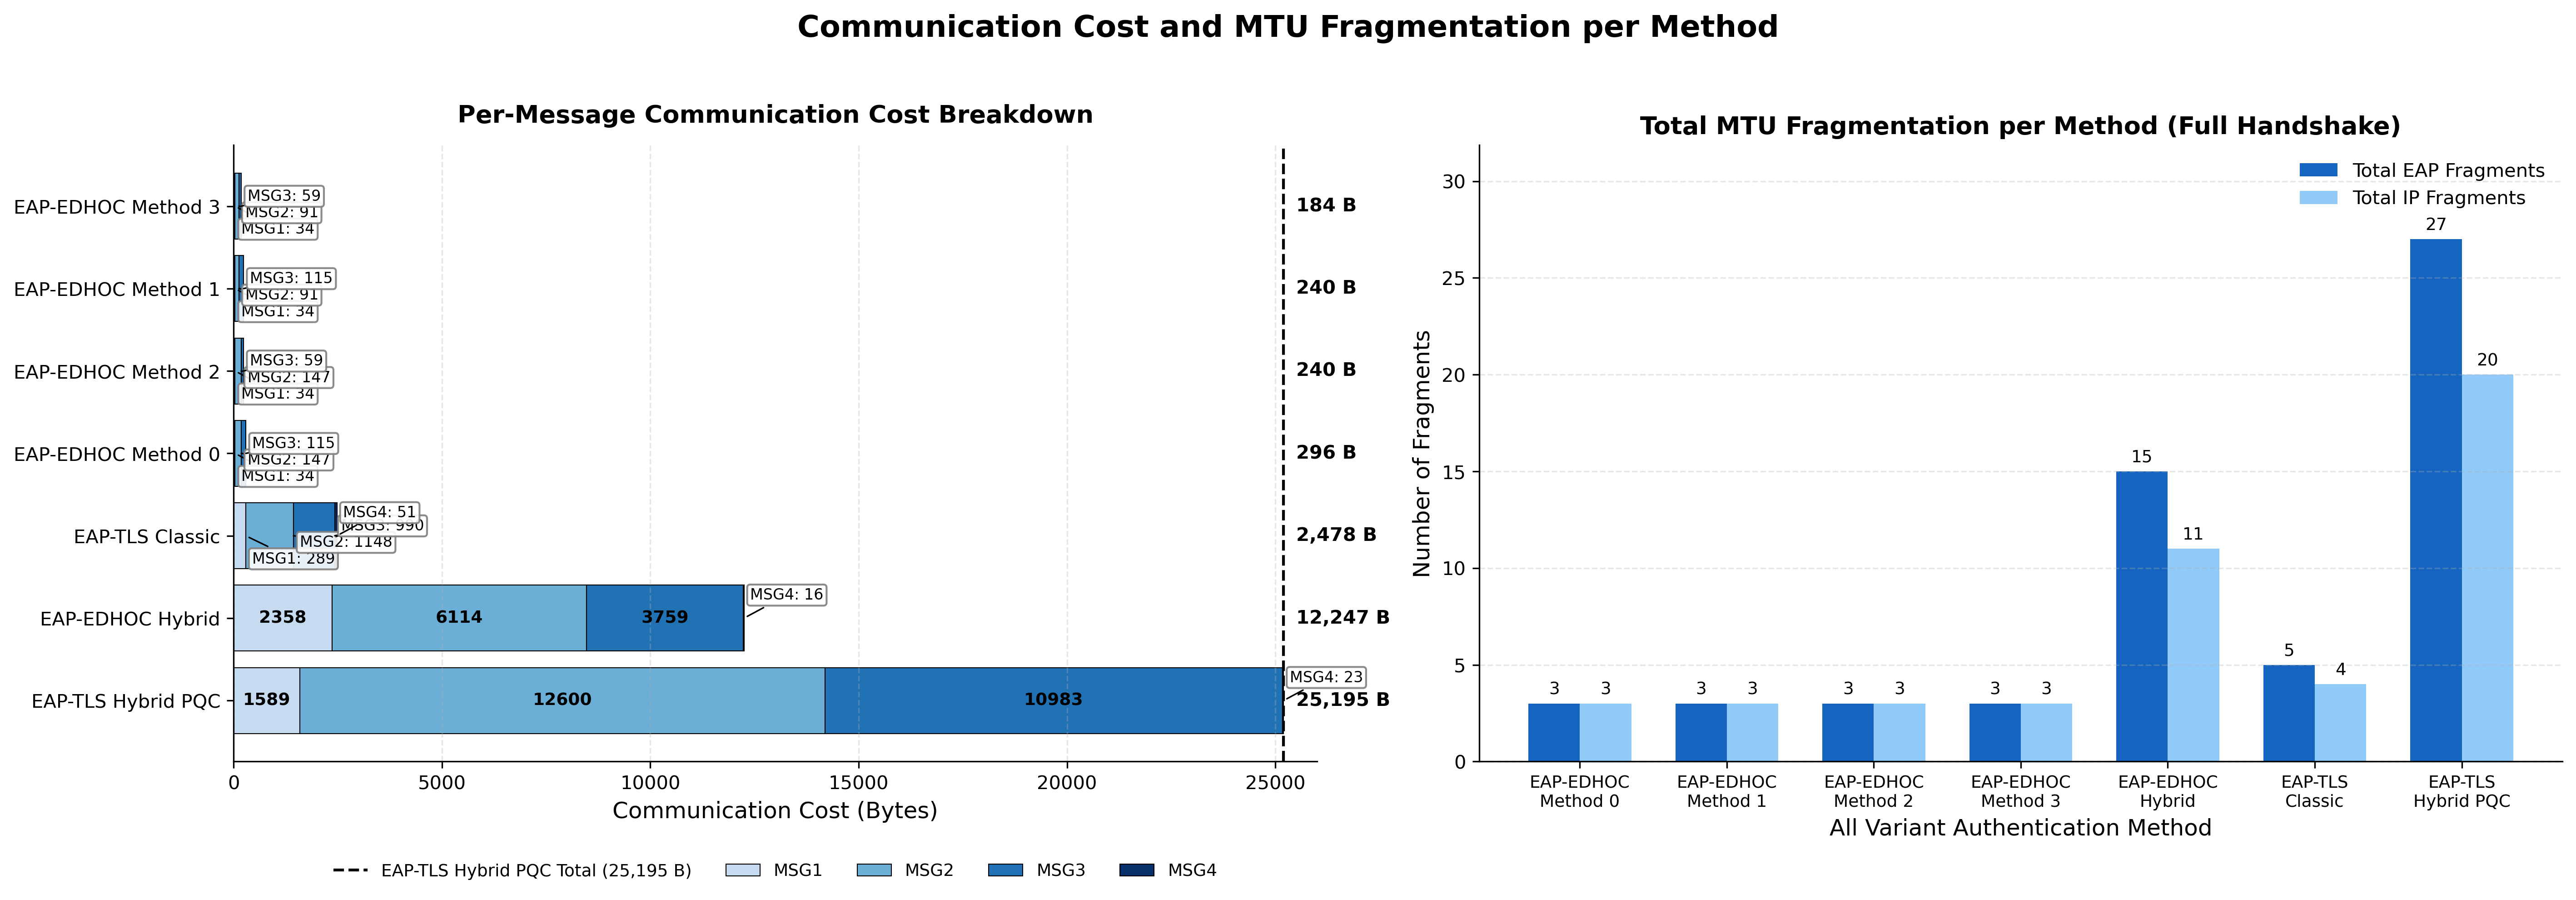
\includegraphics[width=\linewidth]{img_communication_breakdown_methods.png}
\end{adjustwidth}
\caption{Per-method communication (message size) breakdown and MTU fragmentation.\label{fig:communication_breakdown_methods}}
\end{figure}

\subsection{End-to-End Latency, Message Size, and Framing}
Over the live EAP-over-RADIUS path ($100$ iterations per method, no loss), the proposed method completes in $13.223$~ms on average (median $11.946$~ms), against $0.945$--$1.401$~ms for methods 0--3 (medians $0.840$--$0.911$~ms; a few outliers of up to $11$~ms raise their means, and a pooled run of $10{,}000$ handshakes per method in two opposite orders gives medians of $0.987$--$1.033$~ms), $2.699$~ms for EAP-TLS Classic, and $9.696$~ms for EAP-TLS Hybrid PQC. Two costs drive the gap, and neither is computation. The first is fragmentation: the proposal needs $14$ RADIUS round-trips versus $3$ for methods 0--3, and EAP-TLS Classic and Hybrid PQC need $6$ and $28$. The second is durable key rotation: after every run both parties store their rotated one-time keys (write to a temporary file, \texttt{fsync}, atomic rename), and the DN-AAA overwrites and flushes the keys it erases. Tracing $20$ handshakes with \texttt{strace} gives two \texttt{fsync} calls per handshake on the UE and two \texttt{fsync} plus two \texttt{fdatasync} calls on the DN-AAA, where the new record is flushed before \texttt{Message4} is sent (write-ahead). To measure this cost rather than estimate it, we repeated the run with the key directories of both parties on a RAM-backed \texttt{tmpfs}, where the same calls are issued but return almost immediately: the handshake then takes $5.314$~ms on average (median $5.207$~ms, p95 $6.545$~ms) instead of $13.223$~ms (median $11.946$~ms, p95 $24.042$~ms). Durable storage therefore accounts for $7.9$~ms of the mean ($6.7$~ms of the median) on the virtual disk of our VM; on server storage with power-loss protection a flush typically takes well under $0.1$~ms.

The message sizes explain this. Classical messages fit in one EAP fragment ($34$--$147$~bytes). In the proposed method, each X-Wing element adds $1.1$--$1.2$~KB and each ML-DSA-44 signature about $2.4$~KB. \texttt{Message1} ($1{,}141$~B: $ct_B$ and the encrypted \texttt{Plaintext1}) now fits within the $1500$-byte MTU, whereas \texttt{Message2} ($4{,}880$~B) and \texttt{Message3} ($4{,}975$~B) exceed it and are split into EAP fragments (RFC~3579, 253-byte attributes)~\cite{RFC3579} and IP fragments; \texttt{Message4} ($1{,}232$~B) fits in one. The handshake totals $12{,}228$~B. The load per direction is balanced: the UE sends $6{,}116$~B (\texttt{Message1}+\texttt{Message3}) and the DN-AAA $6{,}112$~B (\texttt{Message2}+\texttt{Message4}). EAP-TLS Classic totals $2{,}478$~B in $5$ EAP fragments and EAP-TLS Hybrid PQC $25{,}195$~B in $27$, the most of any method. Cross-implementation checks against pyca/cryptography over OpenSSL passed all $11$ tests, with sizes matching the standards (ML-KEM-768 public key $1184$~B, ciphertext $1088$~B; ML-DSA-44 key $1312$~B, signature $2420$~B).

The two panels of Figure~\ref{fig:handshake_computation_grouped} rank the methods differently, so we compare each EAP-EDHOC variant with the EAP-TLS baseline at the same security level. \emph{Classical pair} (Methods 0--3 vs.\ EAP-TLS Classic, both Ed25519 and X25519): the computation is equal ($0.152$--$0.182$~ms vs.\ $0.182$~ms; we used an Ed25519 certificate instead of RSA-2048 to isolate this effect), yet EAP-EDHOC sends $8$--$13\times$ fewer bytes ($184$--$296$~B vs.\ $2{,}478$~B), needs half the round-trips ($3$ vs.\ $6$), and is $2.9$--$3.2\times$ faster end to end in the median ($0.840$--$0.911$~ms vs.\ $2.651$~ms). \emph{Hybrid PQC pair} (the proposal vs.\ EAP-TLS Hybrid PQC, both X25519+ML-KEM-768 and ML-DSA-44): the proposal computes more ($0.985$ vs.\ $0.775$~ms) because it runs more X25519 and ML-KEM-768 operations, but EAP-TLS carries ML-DSA-44 inside an X.509 chain in a TLS record whereas EAP-EDHOC carries a compact detached CBOR/COSE value, so the proposal again sends half the bytes and needs half the round-trips ($12{,}228$~B and $14$ vs.\ $25{,}195$~B and $28$). Without loss it is nevertheless slower ($13.223$ vs.\ $9.696$~ms mean, $11.946$ vs.\ $9.630$~ms median), because EAP-TLS stores no key material per run; with the key directories on \texttt{tmpfs} the proposal is the faster of the two ($5.314$~ms mean, $5.207$~ms median). Across both pairs, EDHOC's compact encoding, not its primitives, keeps its transport cost below EAP-TLS; for the proposal, forward secrecy without an ephemeral key is paid for in storage flushes instead.

\subsection{Behaviour under Packet Loss}
Figures~\ref{fig:loss_mean} and~\ref{fig:loss_tail} report behaviour under emulated application-level loss with EAP-style retransmission (RTO 40~ms, up to 6 retransmissions per exchange, $120$ trials per cell) for all seven methods. Methods 0--3 keep a $100\%$ success rate up to $10\%$ loss, reach $99.2$--$100\%$ at $20\%$ and $95.8$--$98.3\%$ at $30\%$. EAP-TLS Classic reaches $100\%$ at $20\%$ loss and $96.7\%$ at $30\%$, and EAP-TLS Hybrid PQC $96.7\%$ and $77.5\%$. The proposal reaches $98.3\%$ at $20\%$ loss (mean $390.3$~ms, $8.1$ retransmissions) and $86.7\%$ at $30\%$ (mean $598.2$~ms, $11.3$ retransmissions), between the two EAP-TLS baselines, in line with its $14$ EAP fragments against their $5$ and $27$. Within each security level EAP-EDHOC is the more loss-tolerant: at $30\%$ loss, Methods 0--3 average $116$--$136$~ms against $281$~ms for EAP-TLS Classic, and the proposal $598$~ms with $86.7\%$ success against $1{,}207$~ms and $77.5\%$ for EAP-TLS Hybrid PQC. From $1\%$ loss on, the retransmissions saved by having half the fragments outweigh the fixed storage cost, and the proposal is faster than EAP-TLS Hybrid PQC ($31.9$ vs.\ $34.5$~ms at $1\%$, $88.5$ vs.\ $162.3$~ms at $5\%$). A lost \texttt{Message4} is recovered through the DN-AAA's grace key: in a separate run of $150$ handshakes at $20\%$ loss, one session completed with the retained old key, and all subsequent handshakes succeeded without re-provisioning. Each extra fragment is an independent chance of loss, so latency and retransmissions grow with fragment count. Fragmentation, not computation, is the main scalability concern.

\begin{figure}[H]
\begin{adjustwidth}{-\extralength}{0cm}
\centering
\subfloat[\centering Mean end-to-end latency versus packet loss.\label{fig:mean_latency_loss}]{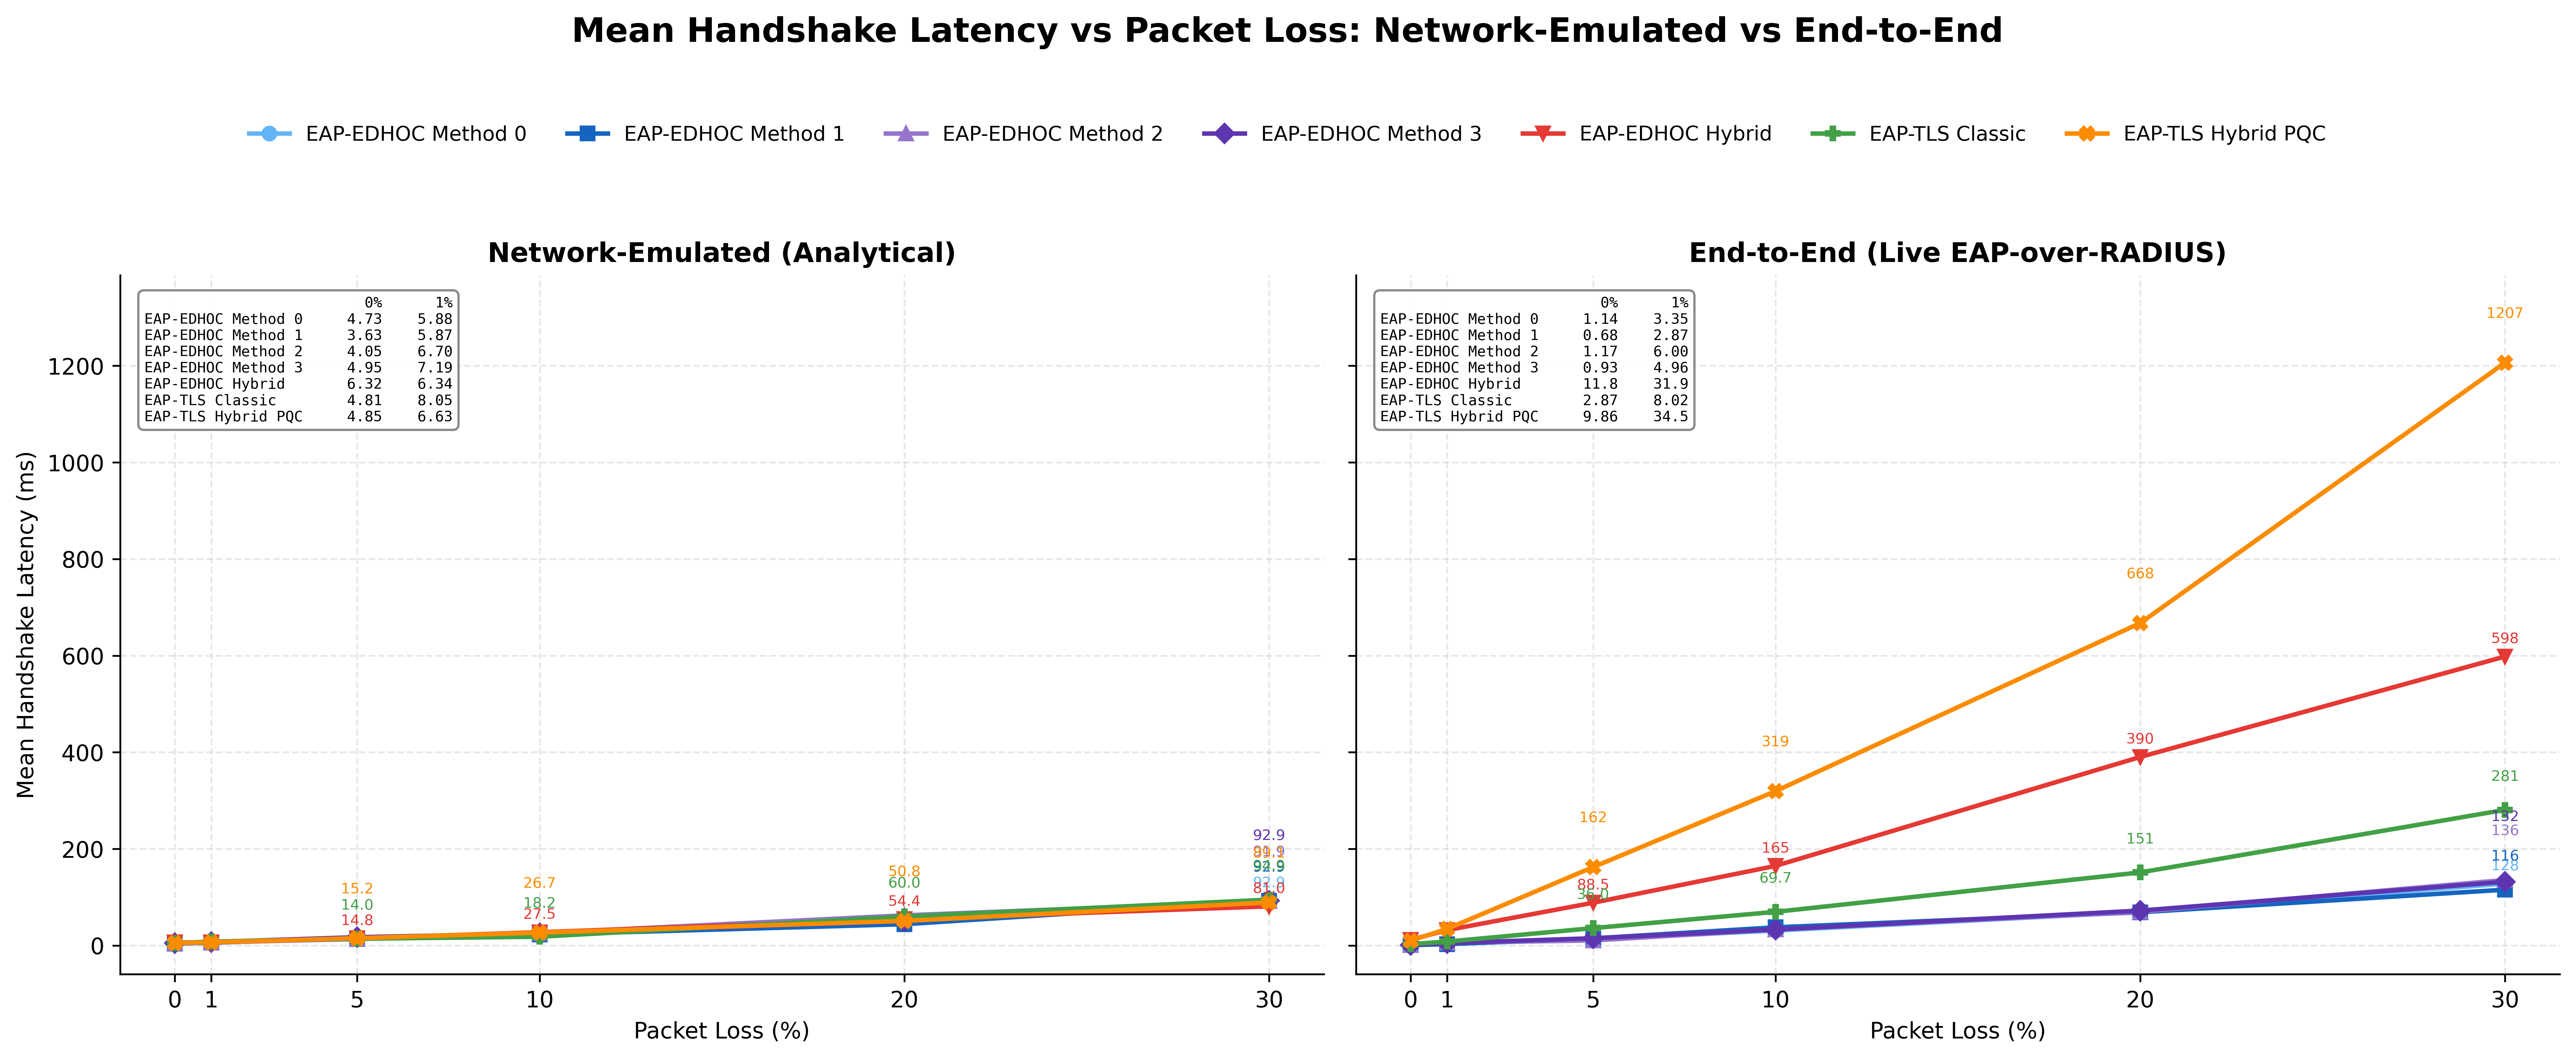
\includegraphics[width=\linewidth]{img_combined_mean_latency_loss.png}}\\
\subfloat[\centering Mean number of retransmissions versus packet loss.\label{fig:mean_Retransmissions}]{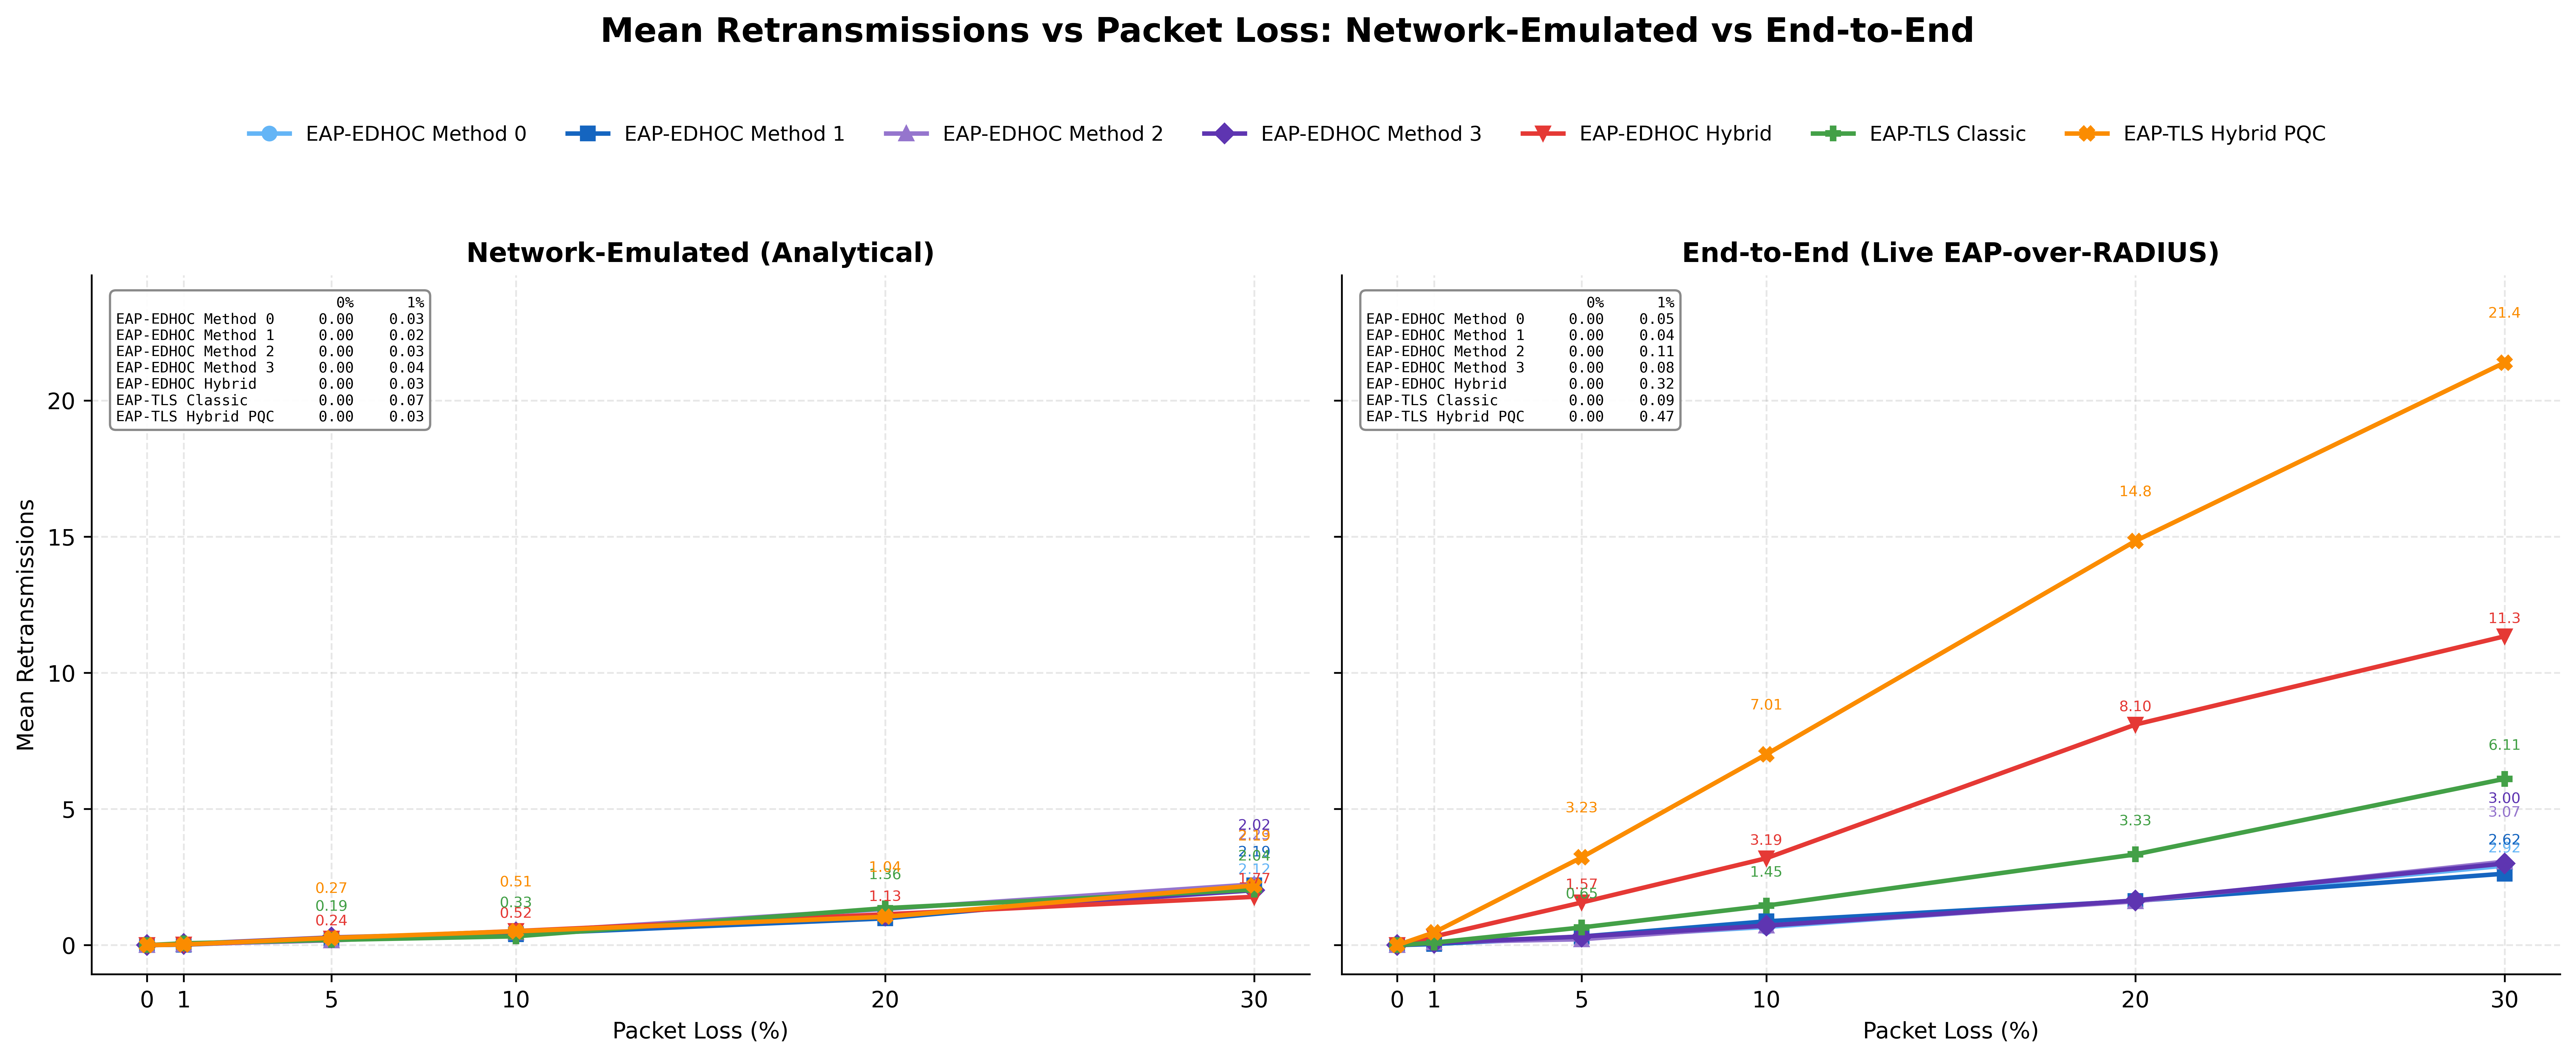
\includegraphics[width=\linewidth]{img_combined_mean_retransmissions.png}}
\end{adjustwidth}
\caption{Mean behaviour under packet loss: (\textbf{a}) end-to-end latency; (\textbf{b}) retransmissions.\label{fig:loss_mean}}
\end{figure}

\begin{figure}[H]
\begin{adjustwidth}{-\extralength}{0cm}
\centering
\subfloat[\centering 95th-percentile end-to-end latency versus packet loss.\label{fig:95th_Percentile_latency_loss}]{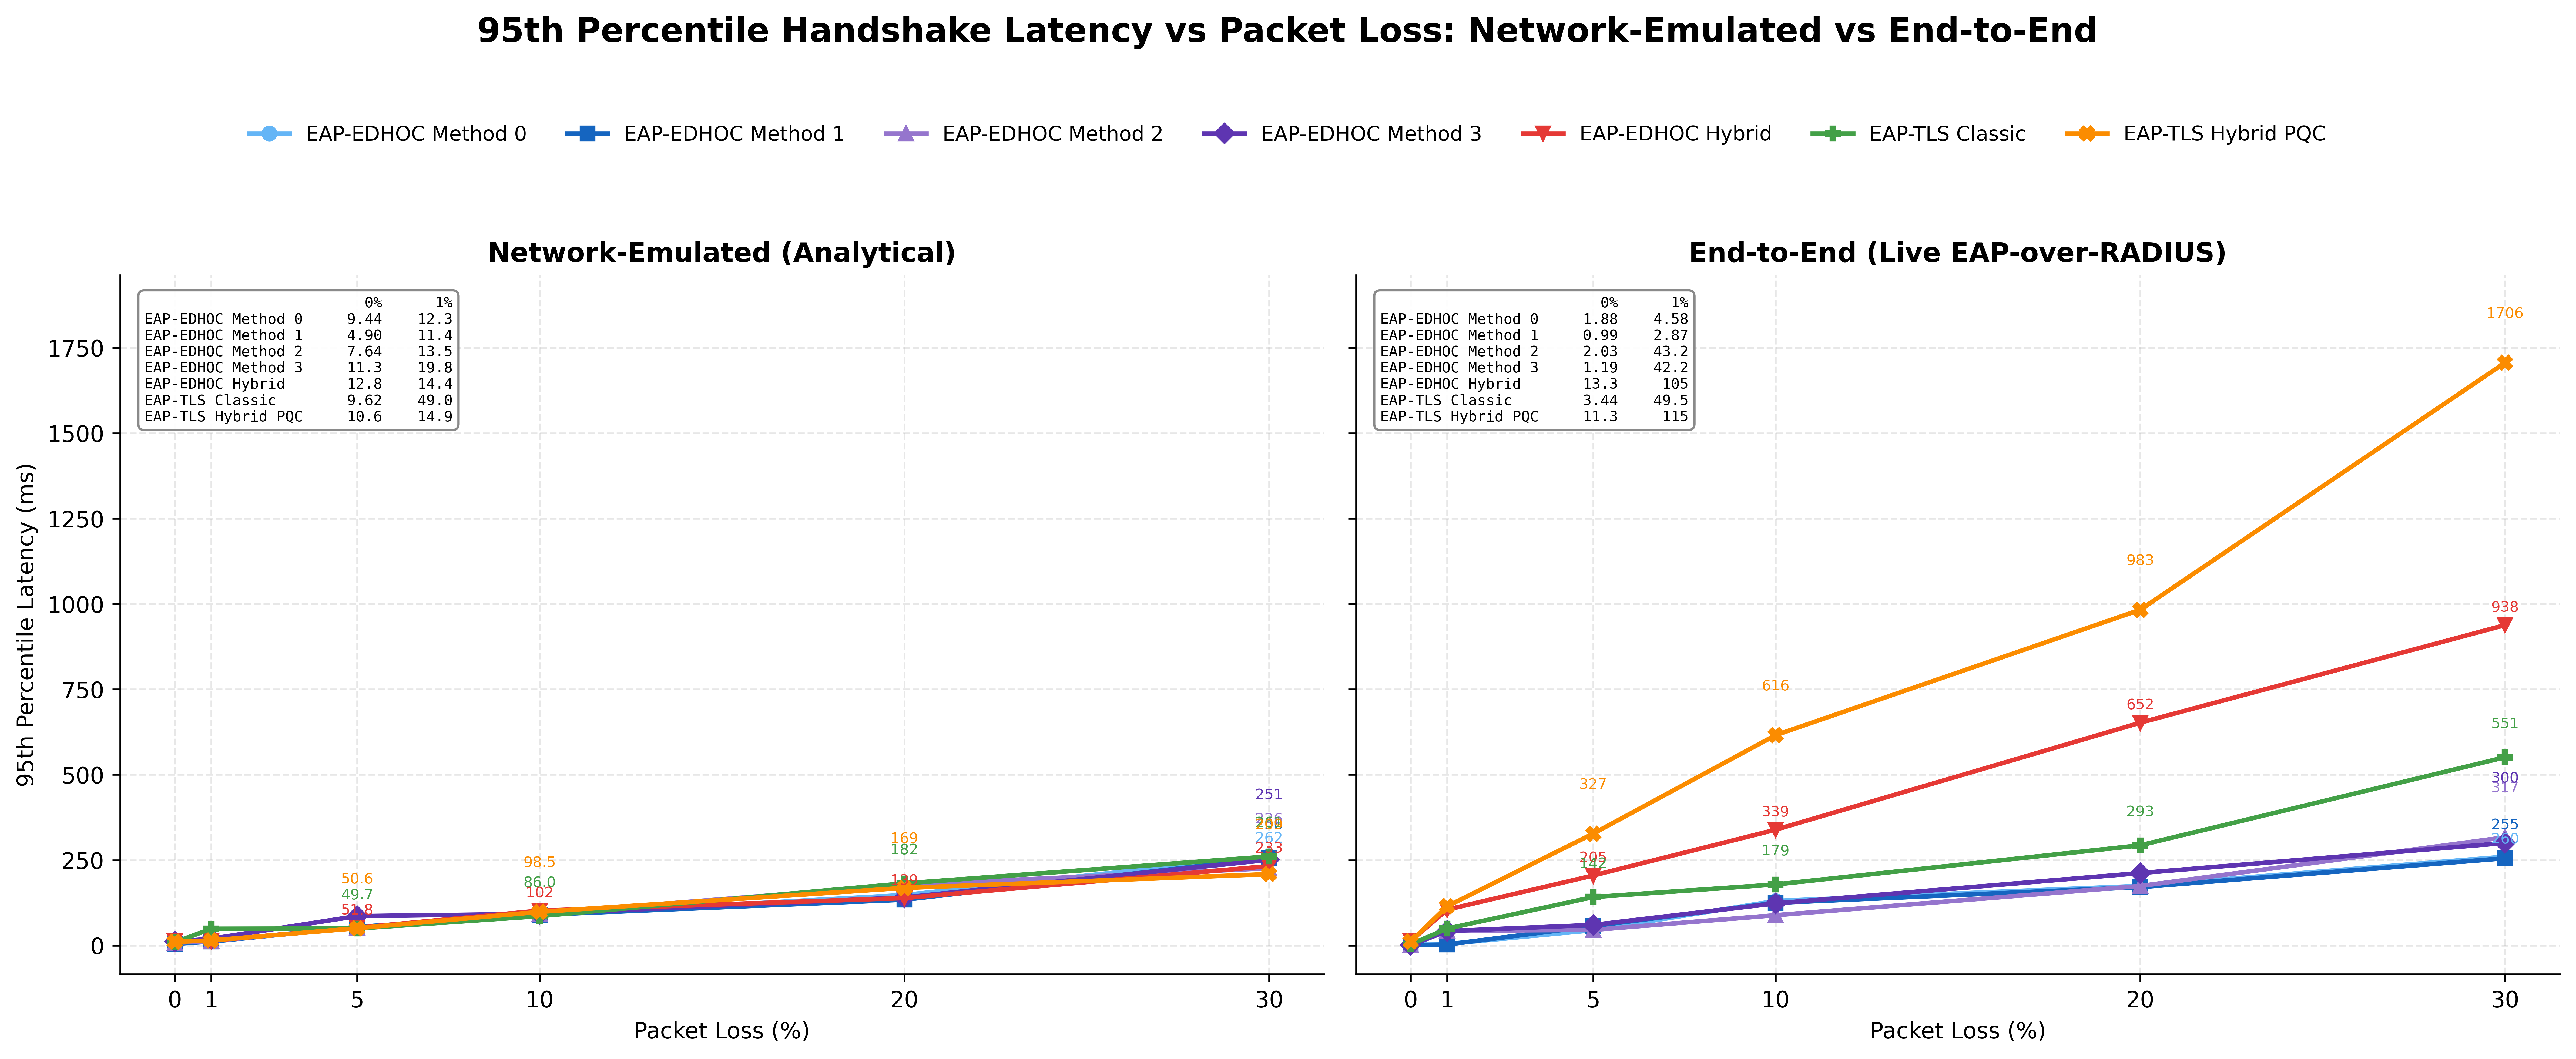
\includegraphics[width=\linewidth]{img_combined_95th_percentile_latency_loss.png}}\\
\subfloat[\centering Handshake success rate across methods and loss levels.\label{fig:success_rate_heatmap}]{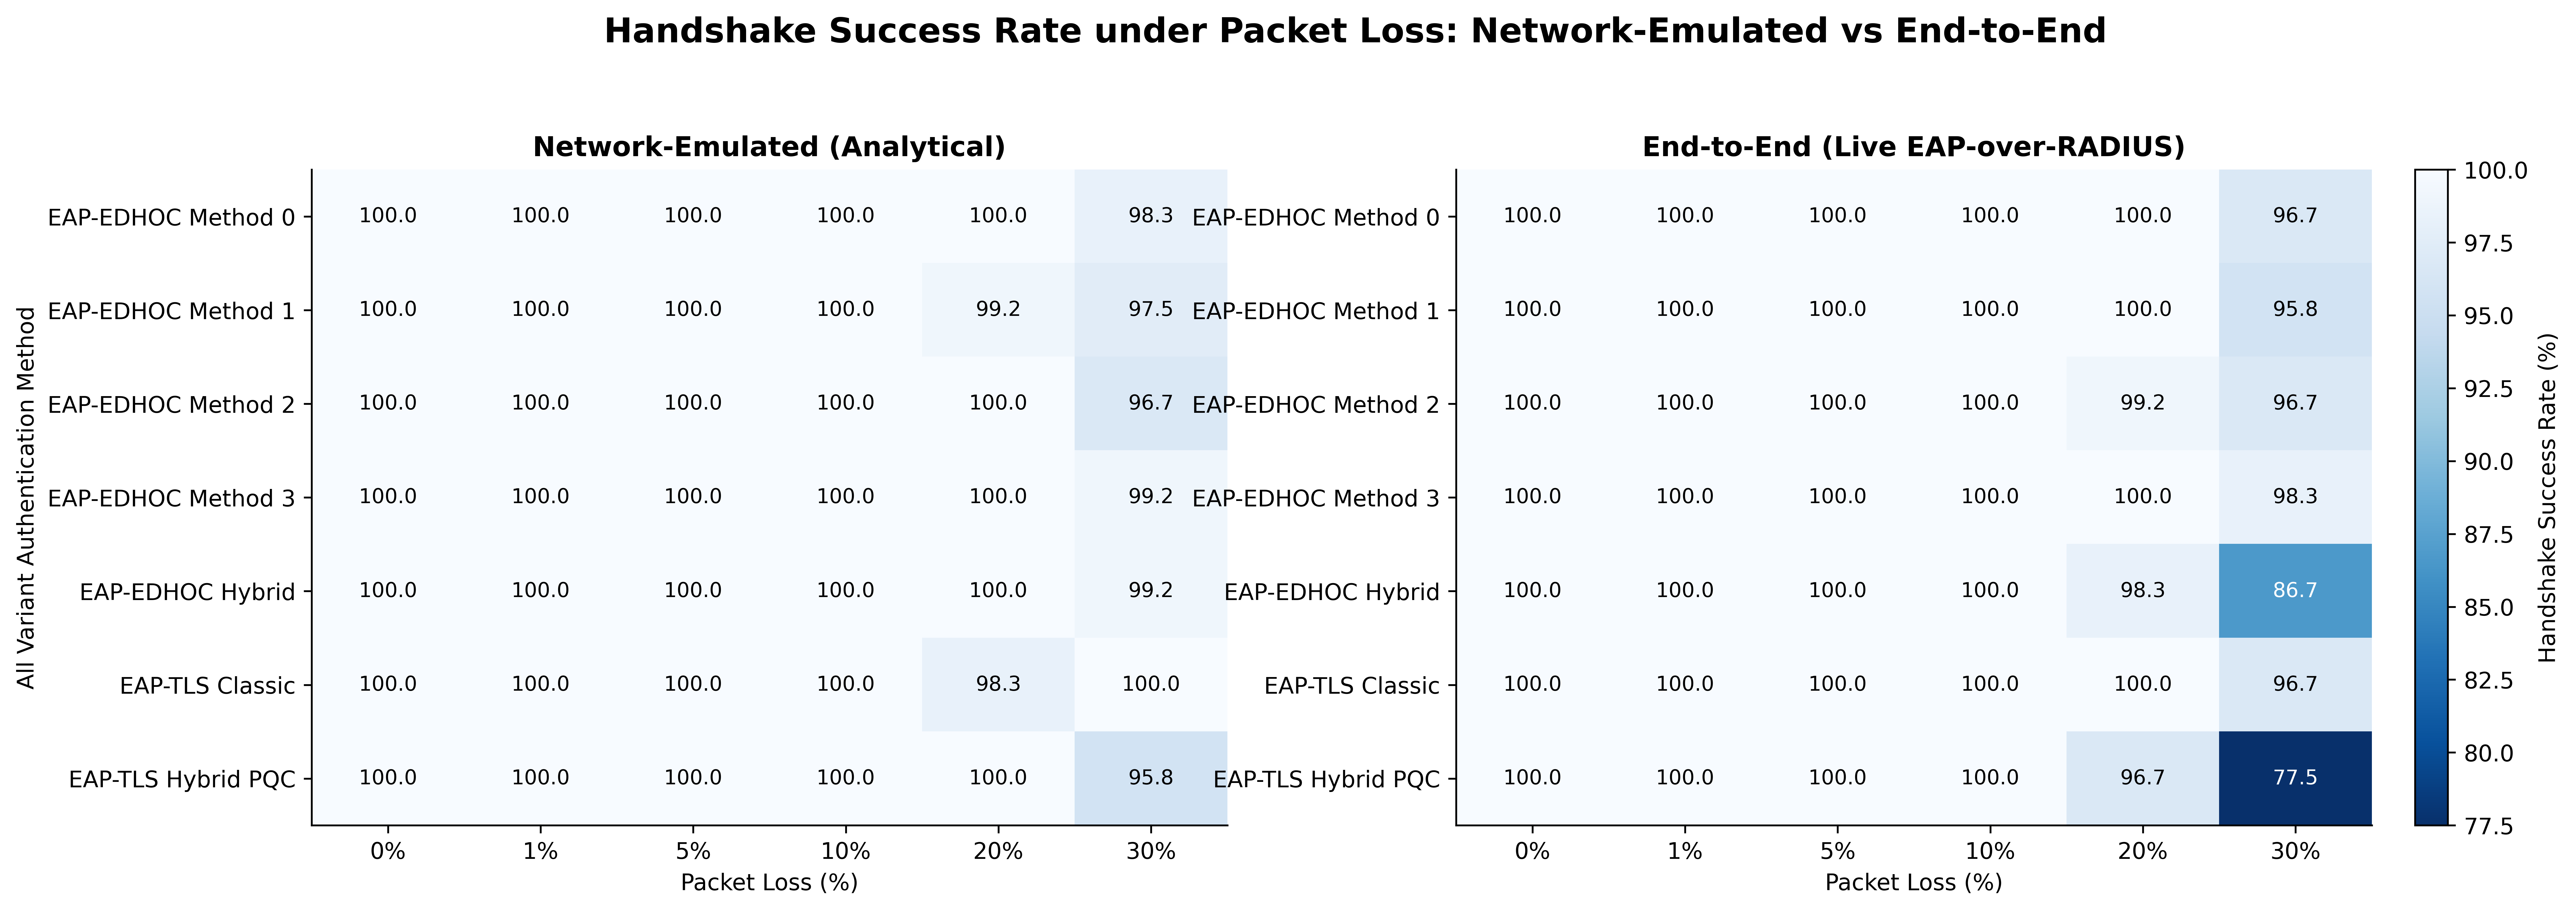
\includegraphics[width=\linewidth]{img_combined_success_rate_heatmap.png}}
\end{adjustwidth}
\caption{Tail latency and reliability under packet loss: (\textbf{a}) 95th-percentile latency; (\textbf{b}) success-rate heatmap.\label{fig:loss_tail}}
\end{figure}



\subsection{EMSK Key-Bootstrapping Cost}
\label{sec:perf-bootstrap}
Every primitive in the bootstrapping chain is inexpensive (Figure~\ref{fig:bootstrap_cost}a), ranging from $0.0012$~ms (OSCORE Master Salt derivation) to $0.0076$~ms (OSCORE Protect, AES-CCM). Of the loss-free end-to-end bootstrap latency of $0.4183$~ms (Figure~\ref{fig:bootstrap_cost}b), only $0.0337$~ms is spent on the four derivation steps (USRK+DSRK on the UE and AAA sides, OSCORE context on the UE and AS sides); the remaining $0.3846$~ms is network overhead on the two new legs, AAA$\to$AS (DSRK transport) and UE$\to$AS (first OSCORE contact). The single-core throughput bound (Figure~\ref{fig:bootstrap_scale}a) is $194{,}481$ sessions/s ($5.142$~\textmu s/session) on the AAA side and $106{,}182$ sessions/s ($9.418$~\textmu s/session) on the AS side, so bootstrapping does not shift the bottleneck away from the AAA server. At $0.42$~ms ($3.2\%$ of the handshake), bootstrapping is far cheaper than the handshake ($13.223$~ms) and far below the $2$--$10$~s typically reported for a manual OAuth~2.0 authorization-code login, at least $4{,}700\times$ faster than the $2$~s lower bound (Figure~\ref{fig:bootstrap_scale}b).

\begin{figure}[H]
\centering
\subfloat[\centering\label{fig:A1_primitive_mean}]{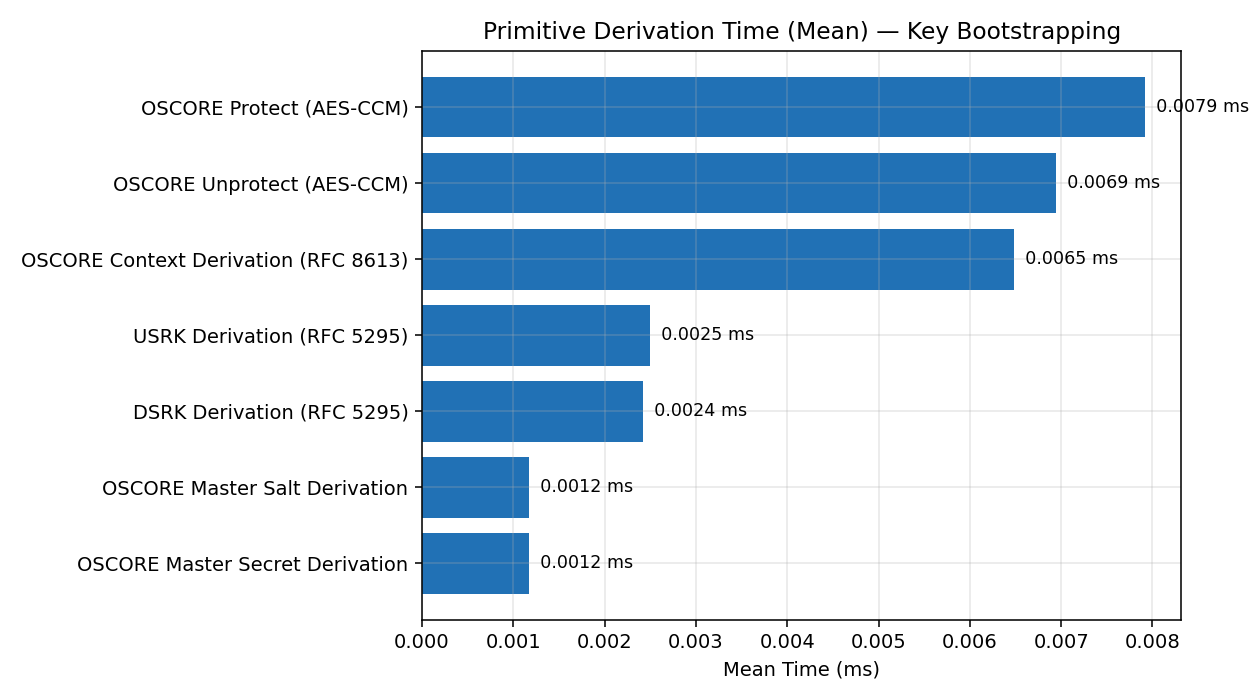
\includegraphics[width=0.49\textwidth]{img_A1_primitive_mean.png}}
\hfill
\subfloat[\centering\label{fig:A2_compute_breakdown}]{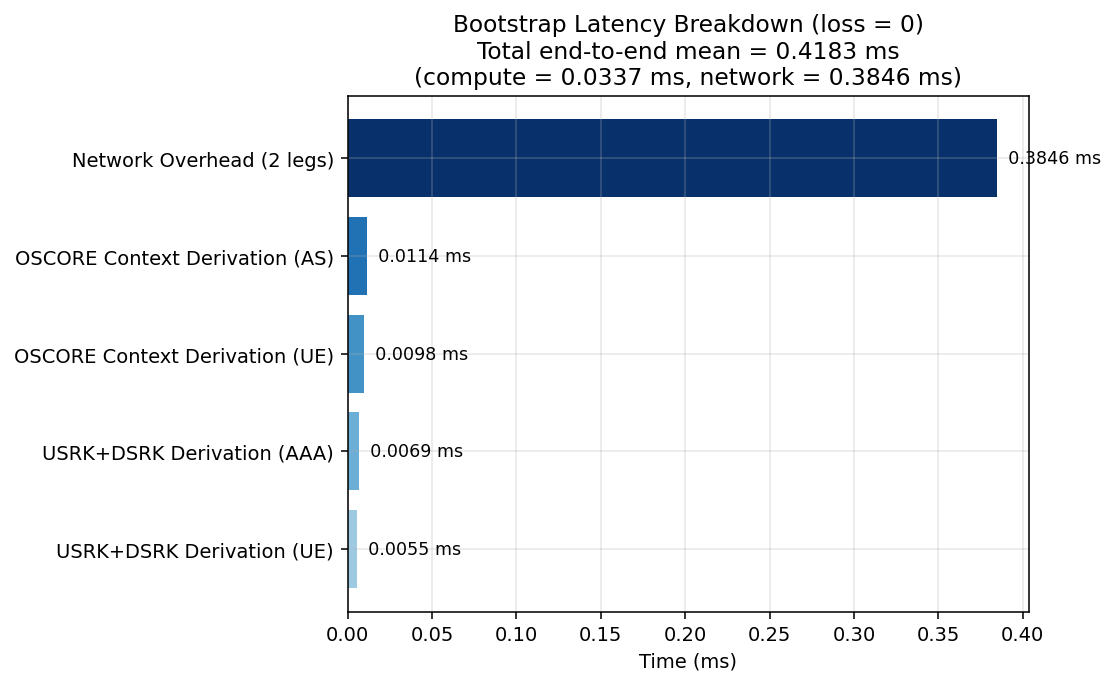
\includegraphics[width=0.49\textwidth]{img_A2_compute_breakdown.png}}
\caption{EMSK bootstrapping cost: (\textbf{a}) mean latency of each primitive; (\textbf{b}) compute and network breakdown of the end-to-end bootstrap.\label{fig:bootstrap_cost}}
\end{figure}

\begin{figure}[H]
\centering
\subfloat[\centering\label{fig:C_throughput}]{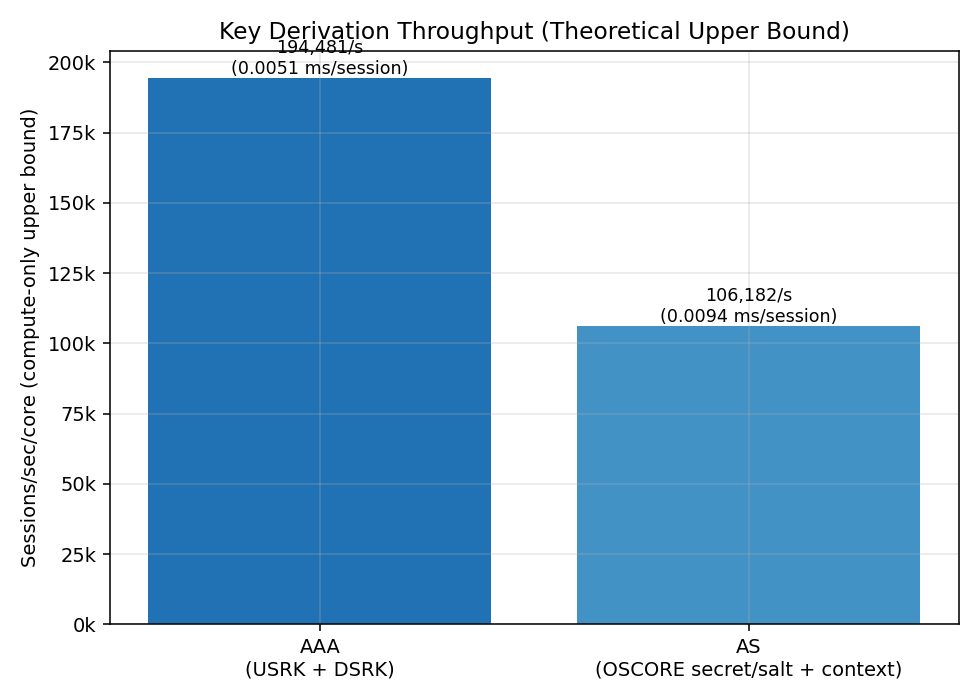
\includegraphics[width=0.49\textwidth]{img_C_throughput.png}}
\hfill
\subfloat[\centering\label{fig:D_baseline_comparison}]{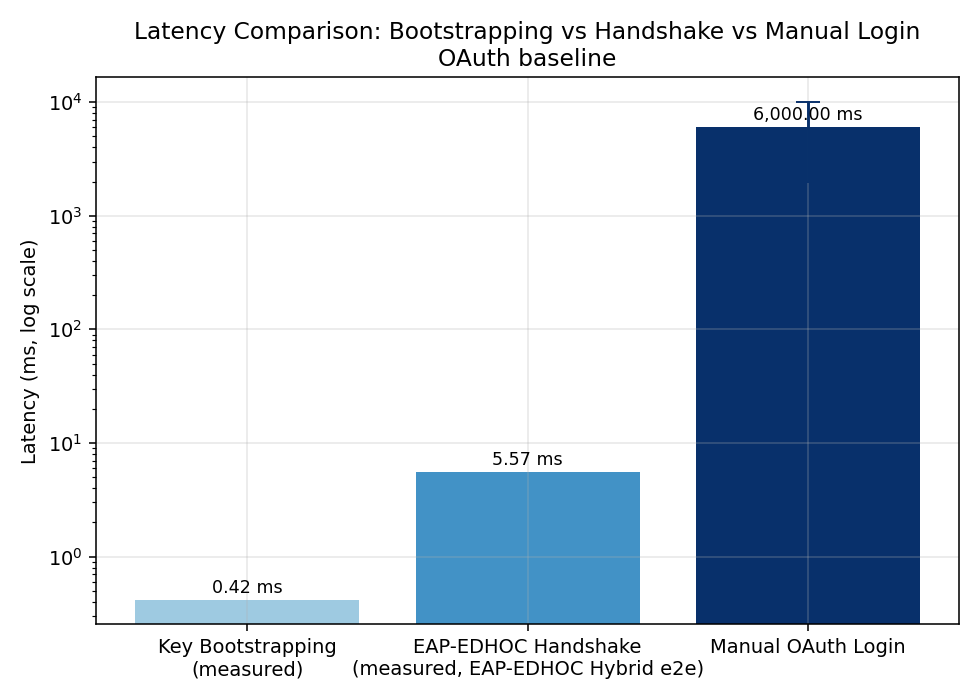
\includegraphics[width=0.49\textwidth]{img_D_baseline_comparison.png}}
\caption{EMSK bootstrapping scalability: (\textbf{a}) single-core throughput; (\textbf{b}) comparison with the handshake and a manual login.\label{fig:bootstrap_scale}}
\end{figure}

Two implementation notes apply. The label \texttt{"dsrk@ietf.org"} is the reserved label of RFC~5295 Section~4, whereas \texttt{"oscore-bootstrap@<specorg>"} for the $ORK$ step is a proposed private-use label (RFC~5295 Section~8), not an IANA registration. Cryptographic separation holds because every level uses distinct labels on the same $\mathsf{Expand}$/$\mathsf{Extract}$ function: compromising $ORK$ in one domain does not reveal another domain's $ORK$, and $DSRK$ does not reveal $EMSK$ (assuming HMAC-SHA-256 is a PRF); $\mathit{id\_context}$ separates multiple OSCORE sessions to the same AS without a new $ORK$. RFC~5295 defines no $DSRK$ transport; RFC~5749~\cite{RFC5749} requires integrity, replay protection, and key wrapping, which we meet with mutual TLS~1.3 between the DN-AAA and the AS, as both sit in one trust domain without an AAA proxy. The chain is purely symmetric and independent of the ML-DSA keys, so its security is inherited from the EMSK.

%%%%%%%%%%%%%%%%%%%%%%%%%%%%%%%%%%%%%%%%%%
\section{Discussion}
\label{sec:discussion}

\textbf{Symmetric guarantees, asymmetric costs.} The results show two distinct symmetry structures. In the \emph{security} dimension the protocol is role-symmetric: both parties are authenticated by independent signatures, both are KCI-resistant, both rotate and erase their one-time keys, and both the computation ($0.492$~ms per party) and the traffic per direction ($6{,}116$ vs.\ $6{,}112$~B) are balanced. In the \emph{cost} dimension it is strongly asymmetric: computation ($0.985$~ms) is under $8\%$ of the $13.223$~ms handshake, and the rest is split between fragmentation over $14$ RADIUS round-trips and the durable storage of the rotated keys ($7.9$~ms on our VM, measured against \texttt{tmpfs}). This decomposition is actionable. Faster PQC primitives would barely change end-to-end latency, whereas the transport cost can be cut today by raising the EAP fragment size or the RADIUS/MTU budget on the SMF--DN-AAA path, and the storage cost by flush-efficient storage or by keeping each key record in a single file, without touching the verified cryptography.

\textbf{Design choices against the closest prior art.} The KEM-based, signature-free method of Fraile et al.~\cite{fraile2025reinventing,pocero} would save the ML-DSA-44 sign/verify cost ($\approx0.223$~ms and $0.060$~ms), which is small against the end-to-end handshake time, while it is precisely the detached signature that gives formally verified KCI resistance independent of the KEM static key (R\ref{req:kci}). It would also break the explicit-authentication symmetry of Section~\ref{sec:symmetry}, since a KEM authenticates only the decapsulator. Shin et al.'s Hybrid-EDHOC~\cite{SIK+25} omits Message~4 to save payload, yet Message~4 is the smallest message ($1{,}232$~B, one EAP fragment; Figure~\ref{fig:communication_breakdown_methods}) and carries the Responder's half of the symmetric key rotation that yields post-compromise security (R\ref{req:pcs}). Omitting it would barely reduce fragmentation, since \texttt{Message2} and \texttt{Message3} dominate the $12{,}228$~B, but would lose a property that T0--T3 lack entirely.

\textbf{Mitigating fragmentation.} Three mitigations require no protocol change: (i) raising the EAP fragment size and RADIUS attribute budget beyond the RFC~3579 253-byte default where the operator controls both endpoints; (ii) raising the path MTU on the SMF--UPF--DN-AAA segment, which never crosses the public Internet; and (iii) adopting more compact PQC parameter sets or signatures as they mature, which would shrink \texttt{Message2} and \texttt{Message3}. None of these affect the authentication logic verified in Section~\ref{sec:formalverif}.

\textbf{Threats to validity.} (1) All components share one VM over loopback, so the network figures are a lower bound; a smaller path MTU or higher RTT in a distributed deployment would make fragmentation more pronounced. (2) Loss is emulated at the application layer rather than with \texttt{netem}, so the relative sensitivity of each method generalises better than the absolute milliseconds. (3) $100$ iterations and $120$ trials per cell separate methods that differ by an order of magnitude but are modest for tail estimates among methods 0--3, whose differences are tens of microseconds (Table~\ref{tab:primitive}). A pooled $10{,}000$-handshake run per method narrows their median confidence intervals to about $\pm3$~\textmu s, but the spread between the fastest and slowest of them is only $45$~\textmu s and their ranking does not follow their compute cost, so we do not rank methods 0--3 against each other. (4) The formal analysis is symbolic, and the quantum adversary is captured by a discrete-log oracle rather than a computational model; a computational proof is future work. (5) Trust in the AAA$\to$AS DSRK channel is a co-location/mTLS assumption analogous to ERP~\cite{RFC6696}, outside the ProVerif model. (6) Forward secrecy now rests on the rotation completing and on the erasure of the old secret keys. If \texttt{Message4} is lost, the UE keeps its old key while the DN-AAA has rotated; keeping the old key for recovery delays forward secrecy for that run, whereas discarding it requires re-provisioning. The models abstract a completed rotation and do not cover this recovery path. Likewise, if the \emph{current} one-time keys of both parties leak before a run, a passive adversary can read that run, since no ephemeral secret remains; security returns from the next run because the rotated secret keys never leave the devices. (7) Re-authentication and handover, including the fate of DSRK/OSCORE state at the AS, are not evaluated.

%%%%%%%%%%%%%%%%%%%%%%%%%%%%%%%%%%%%%%%%%%
\section{Conclusions}
\label{sec:conclusion}
We proposed and implemented a role-symmetric hybrid post-quantum EAP-EDHOC protocol for 5G secondary authentication. X-Wing (X25519 + ML-KEM-768) provides key agreement through exactly two opposite-direction encapsulations to one-time static keys, detached ML-DSA-44 signatures authenticate each party independently of its KEM key, and a two-sided rotation with key erasure provides both forward secrecy and post-compromise security without an ephemeral key pair. ProVerif verification across seven methods shows that only the proposal combines quantum resilience (R\ref{req:qr}), KCI resistance, forward secrecy, and post-compromise security; identity concealment (R\ref{req:idconceal}) holds except under compromise of the Responder's current one-time key before the run. The exported EMSK bootstraps OSCORE keys following RFC~5295 and RFC~8613, so the UE reaches an application server without further login.

On Open5GS, UERANSIM, and FreeRADIUS, the handshake exchanges $12{,}228$~B, split evenly between the two directions, and completes in $13.223$~ms on average, of which $7.9$~ms is durable key storage on our VM. Its cost is asymmetric, concentrated in fragmentation and durable key storage rather than computation; fragmentation dominates under high packet loss. Future work will reduce this overhead through compact PQC parameter sets, EAP fragment-size and MTU tuning, evaluation under mobility and handover with EMSK re-bootstrapping, a computational security proof, and IANA registration of the OSCORE-bootstrap label. Quantum-resistant secondary authentication is thus deployable on existing 5G infrastructure, with security that is symmetric between the parties and a cost that lies in transport and key storage rather than cryptography.

\vspace{6pt}

%%%%%%%%%%%%%%%%%%%%%%%%%%%%%%%%%%%%%%%%%%
% MDPI back-matter statements.
% TODO (authors): items marked [TO BE COMPLETED] must be filled in before submission.
\authorcontributions{Conceptualization, A.P.S.I., S.S. and I.Y.; methodology, A.P.S.I.; software, A.P.S.I., I.W.A.J.P. and H.K.; formal analysis, A.P.S.I. and Y.K.; investigation, A.P.S.I., Y.K., I.W.A.J.P. and H.K.; data curation, A.P.S.I., Y.K., I.W.A.J.P. and H.K.; writing original draft preparation, A.P.S.I. and S.S.; writing review and editing, A.P.S.I. and S.S.; supervision, I.Y. All authors have read and agreed to the published version of the manuscript.}

\funding{This work was supported by the Institute of Information \& Communications Technology Planning \& Evaluation(IITP) grant funded by the Korean government(MSIT) (No. RS-2024-00398312, Development of Quantum Security Based Device Identification and Test Verification Technologies for 5G Non-Public Network)}

\institutionalreview{Not applicable.}

\informedconsent{Not applicable.}

\dataavailability{The source code of the modified Open5GS, UERANSIM, and FreeRADIUS components, the EAP-EDHOC implementation, the ProVerif models, the benchmark scripts, and the raw measurement results supporting this study are openly available in the EdhocSecondaryAuth repository at \url{https://github.com/adipanca/EdhocSecondaryAuth}~\cite{ProVerifSrc}.}

% \acknowledgments{ack}

\conflictsofinterest{The authors declare no conflicts of interest.}

%%%%%%%%%%%%%%%%%%%%%%%%%%%%%%%%%%%%%%%%%%
\abbreviations{Abbreviations}{%
The following abbreviations are used in this manuscript:\\

\noindent
\begin{tabular}{@{}ll}
3GPP & 3rd Generation Partnership Project\\
5G-AKA & 5G Authentication and Key Agreement\\
AAA & Authentication, Authorization, and Accounting\\
AEAD & Authenticated Encryption with Associated Data\\
AMF & Access and Mobility Management Function\\
AS & Application Server\\
AUSF & Authentication Server Function\\
CBOR & Concise Binary Object Representation\\
COSE & CBOR Object Signing and Encryption\\
DN & Data Network\\
DSRK & Domain-Specific Root Key\\
EAP & Extensible Authentication Protocol\\
EDHOC & Ephemeral Diffie--Hellman Over COSE\\
EMSK & Extended Master Session Key\\
HKDF & HMAC-based Key Derivation Function\\
KCI & Key-Compromise Impersonation\\
KEM & Key Encapsulation Mechanism\\
MEC & Multi-access Edge Computing\\
ML-DSA & Module-Lattice-Based Digital Signature Algorithm\\
ML-KEM & Module-Lattice-Based Key-Encapsulation Mechanism\\
MSK & Master Session Key\\
MTU & Maximum Transmission Unit\\
OSCORE & Object Security for Constrained RESTful Environments\\
PQC & Post-Quantum Cryptography\\
RADIUS & Remote Authentication Dial-In User Service\\
SMF & Session Management Function\\
UE & User Equipment\\
UPF & User Plane Function\\
USRK & Usage-Specific Root Key
\end{tabular}
}

%%%%%%%%%%%%%%%%%%%%%%%%%%%%%%%%%%%%%%%%%%
\begin{adjustwidth}{-\extralength}{0cm}

\reftitle{References}

% External BibTeX database (style Definitions/mdpi.bst is selected by mdpi.cls)
\bibliography{egbib}

\PublishersNote{}
\end{adjustwidth}
\end{document}
